\documentclass[12pt]{report}
\usepackage{graphicx}
\usepackage[section]{placeins}
\usepackage{amsmath,amssymb,latexsym} 
\usepackage{wrapfig}
\usepackage{lscape}
\usepackage{rotating}
\usepackage[margin=1in]{geometry}
\graphicspath{ {images/} }

\begin{document}


\tableofcontents
\listoffigures

\chapter{Introduction}\label{ch:introduction}
\addcontentsline{toc}{chapter}{Introduction}
Matrimonial sites in India operate on the basis of bringing in technology to facilitate what was so far known as an arranged marriage. The astounding growth of online matrimonial sites is largely because of numerous choices they offer to its users, making it very convenient for them to find a suitable partner.

Matrimonial websites are a big business because they blend in the traditional with the modern. Traditional families are happy that these sites offer them the choice of caste, creed, and other such parameters which they would otherwise look for in a prospective bride/groom; on the other hand, the huge database offers young people the chance to browse for someone based on their tastes, and then filter it down to someone they think they could connect to.

Keeping this objective in mind , a reliable match-making service with the help of database management system has been created.




\section{Purpose}
The purpose of this project is to design a database system to facilitate a matrimonial matchmaking service. The existing system is yet to fully evolve as the current generation need a better and a more reliable and user-friendly experience as compared to the old players of the previous generations. 
The intent of the project is to gather and maintain data pertaining to each individual with the required queries and to design an effective front-end application to implement the same, keeping the objective of optimizing risk management and control in mind. 


\section{Scope}
The proposed system will allow every user to sign up on the website by filling out a few mandatory details. All the details can be edited as and when required. After signing up users will be able to filter other profiles based on what they are looking for. \\\\
All details of a user is not available to be viewed by everyone. When a user wants to view the profile of another user, an access request needs to be sent. Once the other user approves, the profile can be viewed. \\\\
Users can contact other users from within the website by sending messages to them. The messages can be replied to as well as deleted from the database.\\\\
If a user wishes to deactivate his/her profile for a while, they can do so. Their data will still be available on the database but their profile can neither be viewed nor searched for. \\\\
If a user wishes to delete his profile completely, he can do so. All the data he has uploaded will get erased completely. \\\\
If a match is made and a couple decides to get married they can update their story on the website under Success Stories.   



\chapter{Software Requirements Specification}\label{ch:srr}

\section{Overall Description}
A software requirements specification (SRS) is a document that captures complete description      
about how the system is expected to perform. It is a comprehensive description of the intended purpose and environment for software under development.\\\\
To be used efficiently, all computer software needs certain hardware components or other software
resources to be present on a computer. These prerequisites are known as (computer) system
requirements and are often used as a guideline as opposed to an absolute rule. Most software defines
two sets of system requirements: minimum and recommended.

\section{Specific Requirements} 

\subsection{Software Requirements}

\begin{itemize}
\item Operating Systems
\begin{itemize}
\item Client Side : Any OS with a suitable web browser. 
\item Server Side : Any Linux Server Distribution

\end{itemize}

\item Database: MySQL 
\item  Server scripting: Python’s Flask framework
\item Front End Interface: HTML, CSS, Javascript and JQuery
\end{itemize}

Consequently to run the database application a suitable browser compatible with all of the aforementioned requirements is necessary. Speculated ones are Google Chrome, Mozilla Firefox.




\subsection{Hardware Requirements}
\begin{itemize}
\item \textbf{Server Side :} The system will be hosted online with help of hosting services like AWS, Google Cloud Platform or Microsoft Azure. 

\item\textbf{Client Side :}   Any device with an Internet connection and a suitable web browser that supports HTML 3 or above. 
\end{itemize}



\subsection{Functionality}
Functional Requirements explain the main and important features of the Database Management Systems and how they can be used by the clients and users to achieve the purpose. Functional Requirements can include technical details, and specific personality that can help accomplish the purpose of the Database Management System.

\begin{itemize}

\item \textbf{Adding new users}\\ Matrimonial Database Management System should be able to allow addition of new users to the Database and each new user is will choose a unique Username at the time of his/her registration.
 
 
\item \textbf{Adding User Mandatory Information}\\
Each user shall have the following mandatory information: first name, last name, gender, date of birth and image. 

\item \textbf{Update/Modify User Information}\\
The matrimonial database management system shall allow the user to update any of the user’s information.

\item \textbf{Delete User Information}\\Information which is not mandatory can be deleted by the user at any point of time. 

\item\textbf{Searching for Matches} \\Each user should be able to search the database for a match, based on filters on the various attributes. 

\item\textbf{Requesting for Access to View Profile}\\
Each user can send a ‘View Profile’ request to other users. If accepted they can view their entire profile, else they can view only basic details. 


\item\textbf{Messaging System} \\Each user can send messages to other users. 

\item\textbf{Deactivate/Delete Account} \\Each user can deactivate his/her account at any point of time. This will render his profile inaccessible. 
Each account can also be deleted completely, which will remove all the data from the database. 

\item\textbf{Adding Success Stories} \\If a user finds a match using the website and decides to get married, they can add a success story. This story can be viewed by the other users. 


\end{itemize} 


\subsection{Non-Functional Requirements}
\begin{itemize}

\item\textbf{Security } \\The system requires the User to identify himself/herself using a unique \emph{username.} 
\begin{itemize}
\item\textbf{Login ID } \\Any user who uses the system shall have a Username and Password. 

\item\textbf{Modification} \\Any modification (insert, delete, update) for the Database shall be synchronized. 


\end{itemize}

\item\textbf{Portability } \\Since it is a web based application, it can be used on any device with a browser.

\item\textbf{Reliability} \\Constraints are enforced to ensure the consistency of the data throughout. 

\end{itemize}


\chapter{Detailed Design}
\paragraph*{•}
A data flow diagram is a graphical representation of the "flow" of data through an information system, modeling its process aspects. A DFD is often used as a preliminary step to create an overview of the system without going into great detail, which can later be elaborated. DFDs can also be used for the visualization of data processing. DFD is a designing tool used in the top-down approach to Systems Design. \\

Using any convention’s DFD rules or guidelines, the symbols depict the four components of data flow diagrams:

\begin{enumerate}
\item \textbf{External entity} \\An outside system that sends or receives data, communicating with the system being diagrammed. They are the sources and destinations of information entering or leaving the system. They might be an outside organization or person, a computer system or a business system. They are also known as terminators, sources and sinks or actors. They are typically drawn on the edges of the diagram.

\item \textbf{Process} \\ Any process that changes the data, producing an output. It might perform computations, or sort data based on logic, or direct the data flow based on business rules. A short label is used to describe the process, such as “Submit payment.”

\item \textbf{Data store} \\Files or repositories that hold information for later use, such as a database table or a membership form. Each data store receives a simple label, such as “Orders.”

\item \textbf{Data flow} \\The route that data takes between the external entities, processes and data stores. It portrays the interface between the other components and is shown with arrows, typically labelled with a short data name, like “Billing details.”

\end{enumerate}


\section{DFD Level 0}

The level zero of the data flow diagram represents only the actions and responses of the database involving the users. The user can request for any kind of data from the database. The database can respond with the available data or give an appropriate response if the data is not available. 


\begin{figure}[!htb]
    \centering
    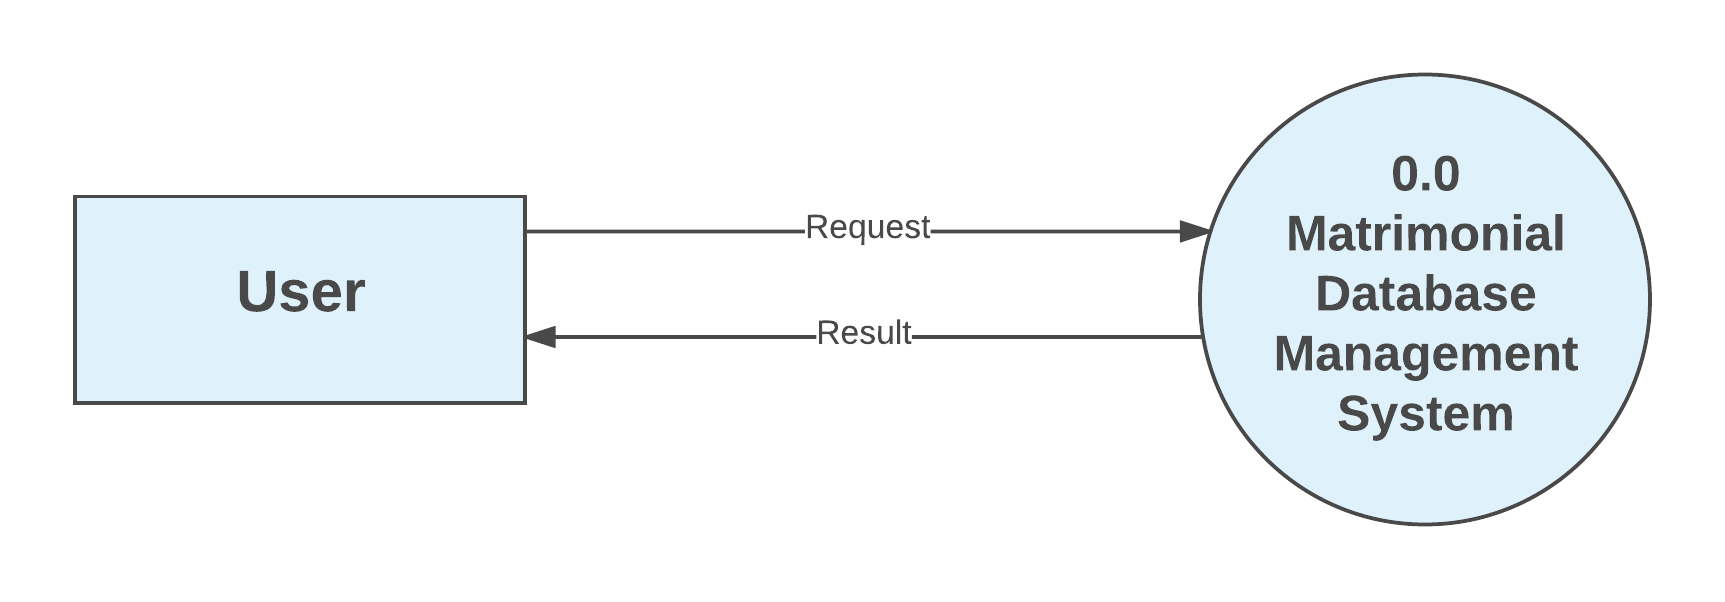
\includegraphics[width=1\textwidth]{df-l0.png}
    \caption{DFD Level 0}
    \label{fig:dfd l0}
\end{figure}


\section{DFD Level 1}

The level one of the Data Flow Diagram of the Matrimonial Database System depicts the different functionalities a user has. These are insertion, deletion, modification, searching, messaging, requesting for user access and viewing profiles.

\begin{itemize}
\item\textbf{Insertion} \\ Involves adding data to the various tables in the database.

\item\textbf{Deletion} \\Involves removing all the data of a particular user from the database.  

\item\textbf{Modification} \\Involves modifying the data from the different tables.

\item\textbf{Searching} \\Involves two types of searching, quick search and advanced search. In quick search the profile can be viewed directly by providing the username. In advanced search, various filters can be applied and user profiles are shown appropriately. 

\item\textbf{Messaging} \\Involves sending and replying to messages between users. 

\item\textbf{Requesting User Access } \\ Involves sending requests to the users to ask for access to view their details. 

\item\textbf{Viewing Profiles } \\ Involves viewing the profiles of other users. 

\item\textbf{Viewing Success Stories } \\ Involves viewing the successfully matched profiles and the users' experiences on the website. 


\end{itemize}

 

\begin{figure}[!htb]
    \centering
    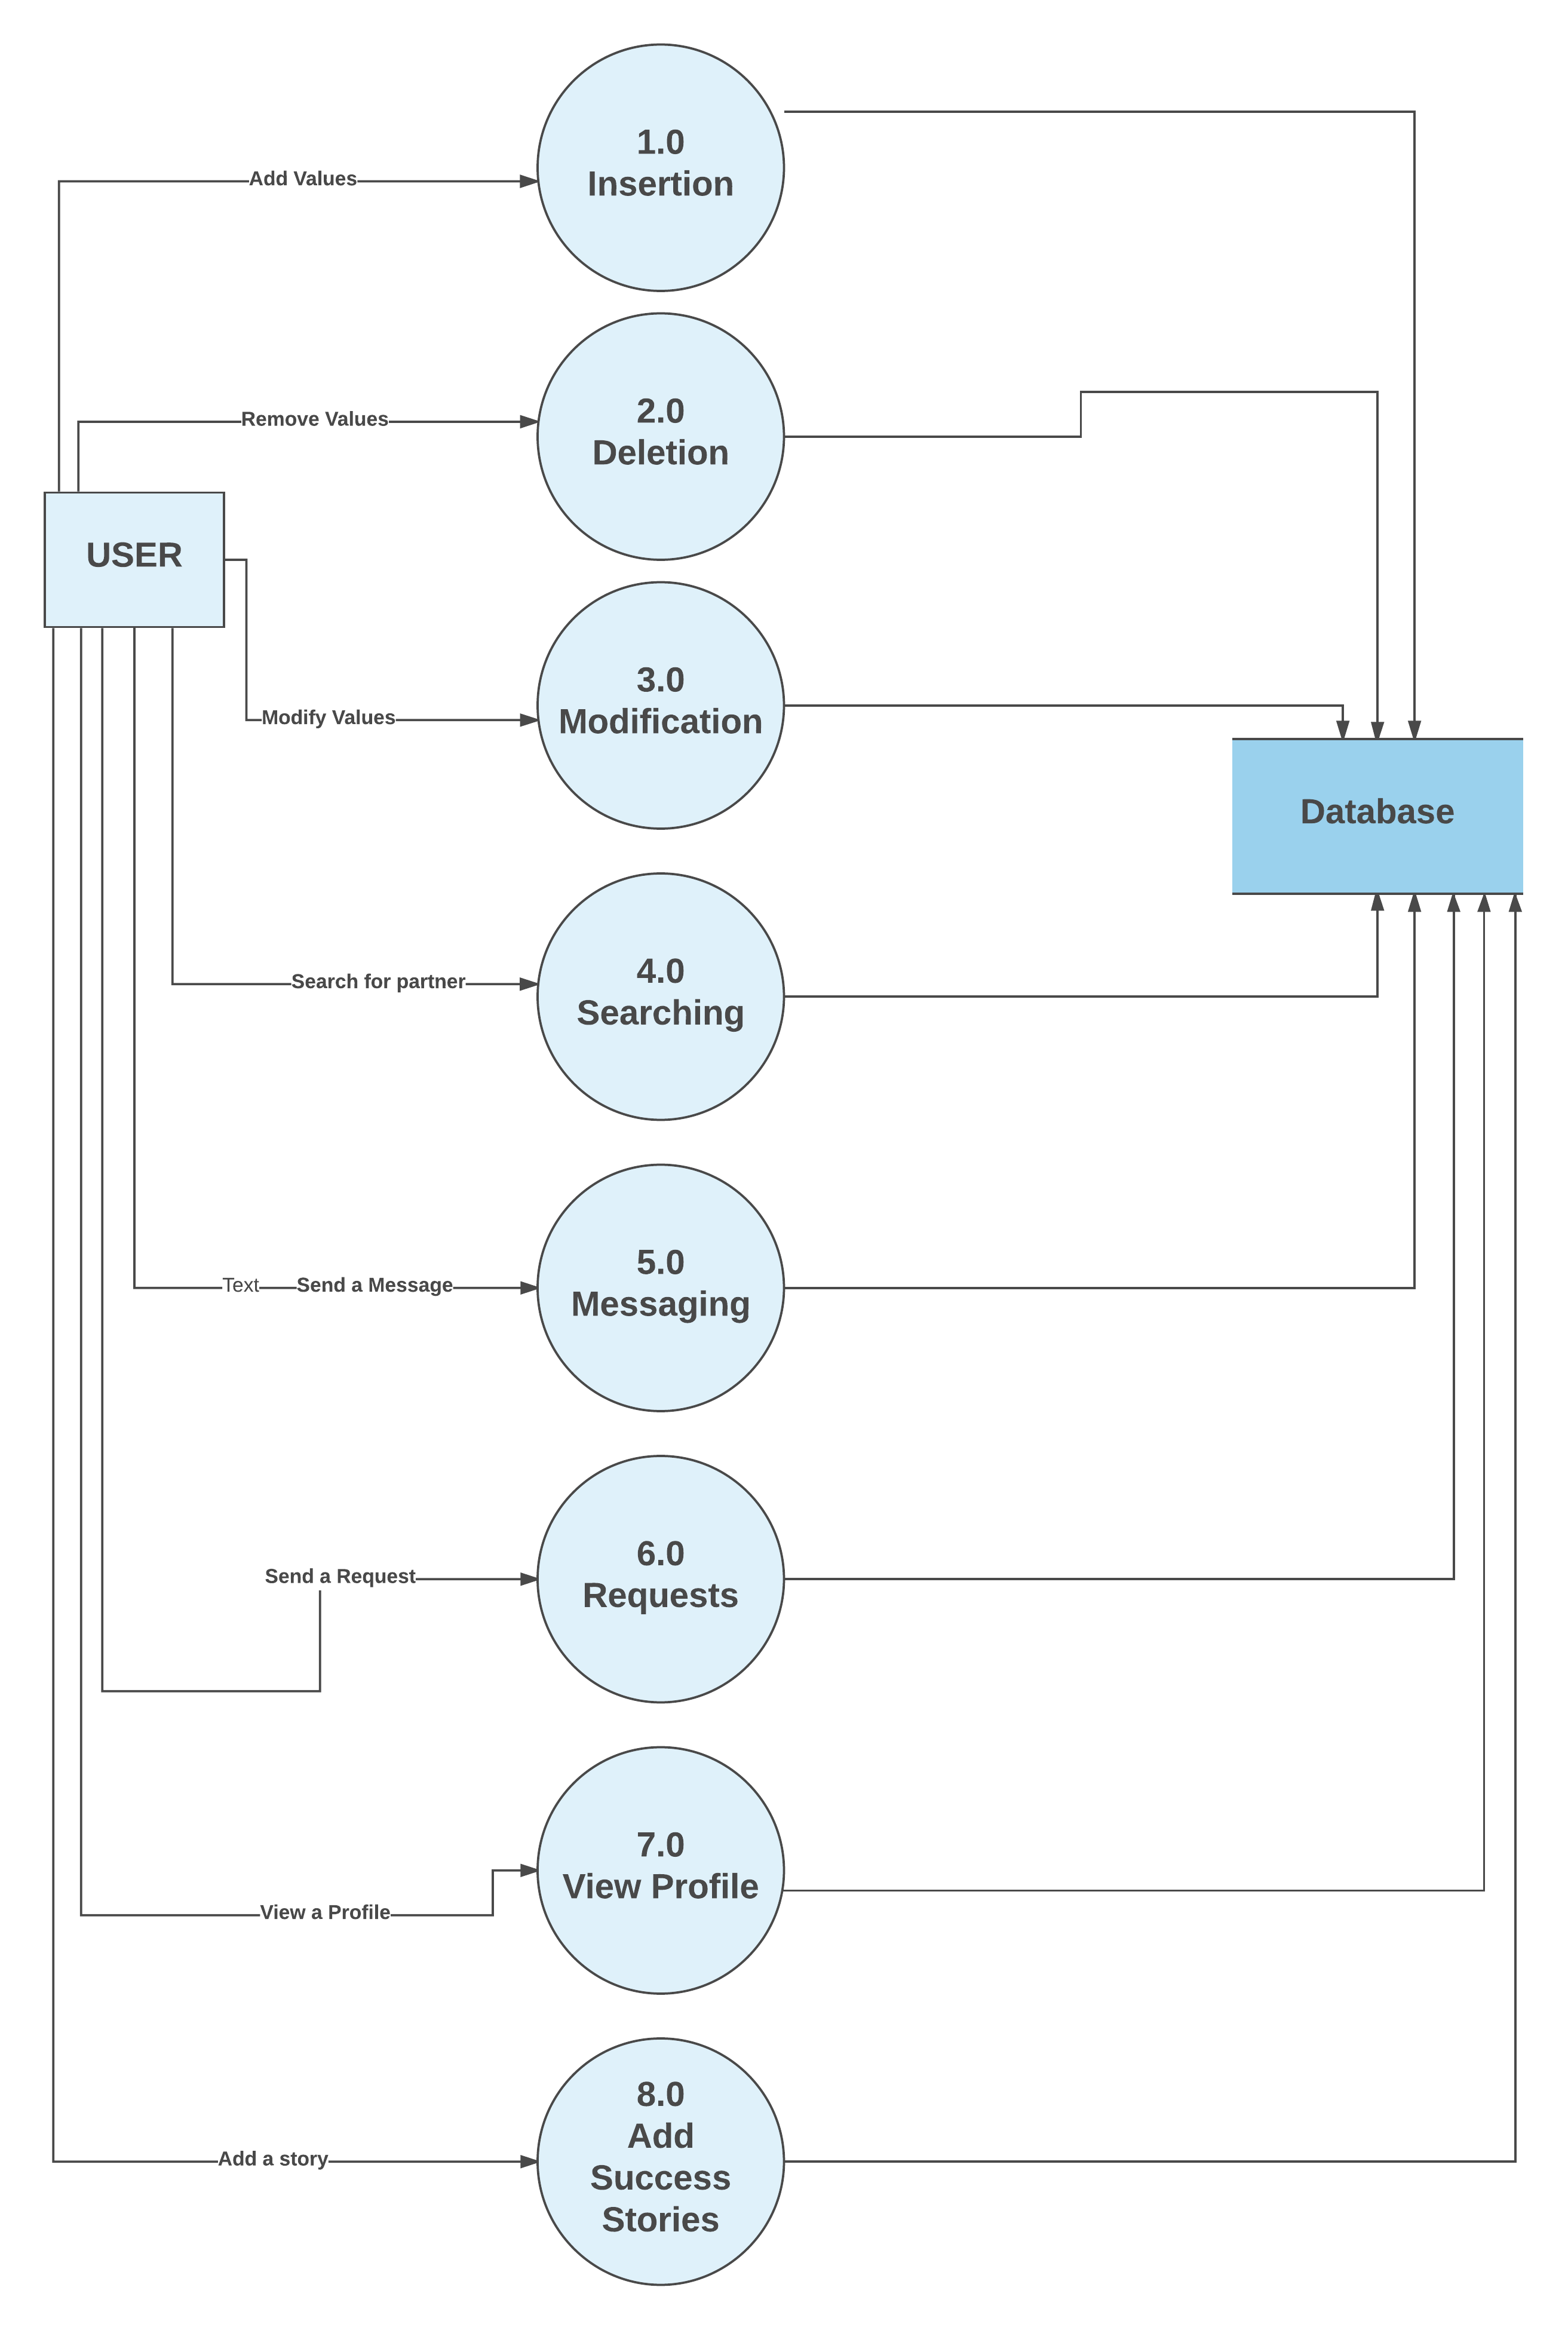
\includegraphics[width=.7\textwidth]{df-l1.png}
    \caption{DFD Level 1}
    \label{fig:dfd l1}
\end{figure}



\section{DFD Level 2}
The level two of the DFD splits each task in level 1 into separate diagrams for a much more detailed description of the data flow. Each process can be shown as follows: 



\begin{figure}[!htb]
    \centering
    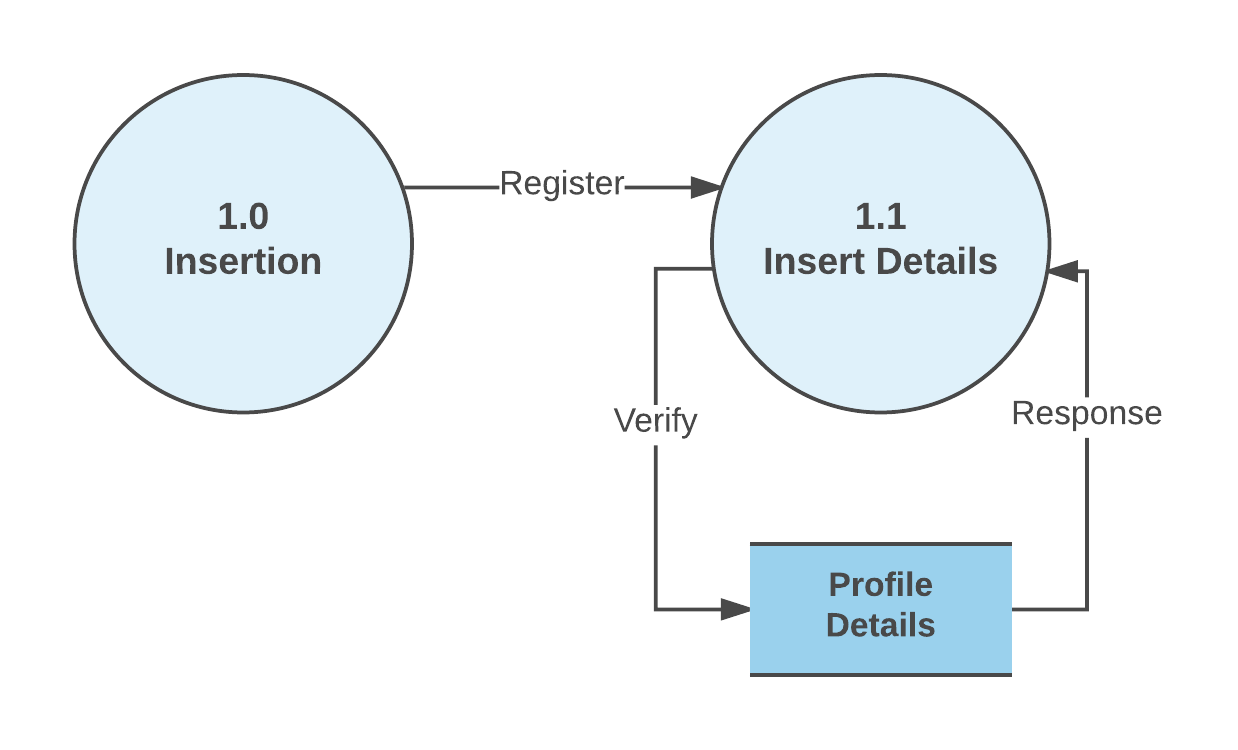
\includegraphics[width=.8\textwidth]{df-l2-1.png}
    \caption{DFD Level 2.1}
    \label{fig:dfd l2.1}
\end{figure}

\begin{figure}[!htb]
    \centering
    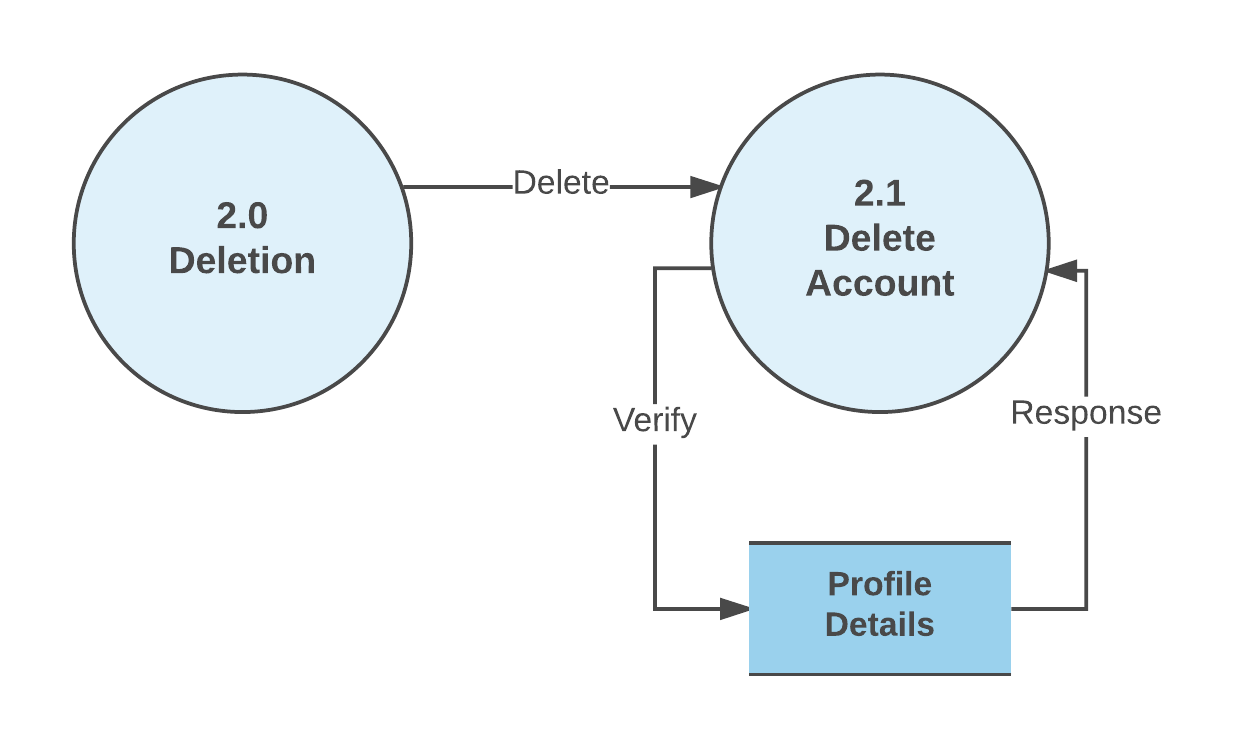
\includegraphics[width=.8\textwidth]{df-l2-2.png}
    \caption{DFD Level 2.2}
    \label{fig:dfd l2.2}
\end{figure}

\begin{figure}[!htb]
    \centering
    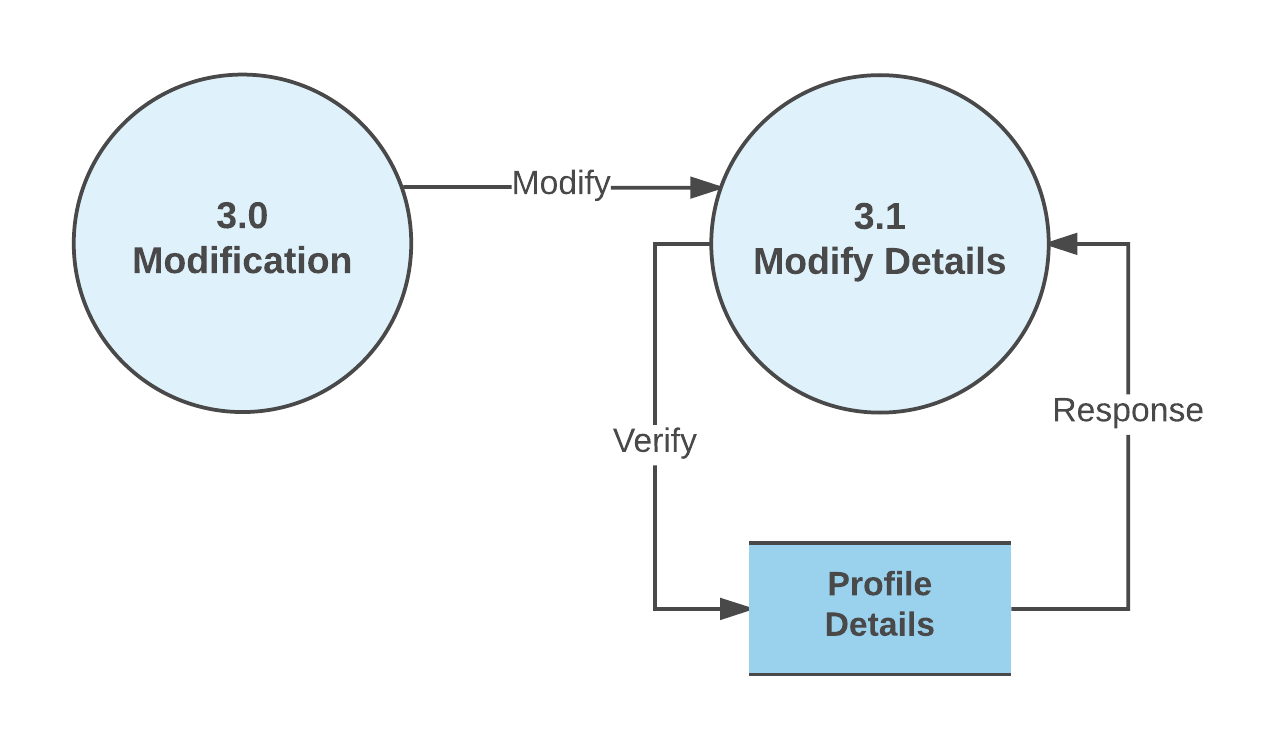
\includegraphics[width=.8\textwidth]{df-l2-3.png}
    \caption{DFD Level 2.3}
    \label{fig:dfd l2.3}
\end{figure}

\begin{figure}[!htb]
    \centering
    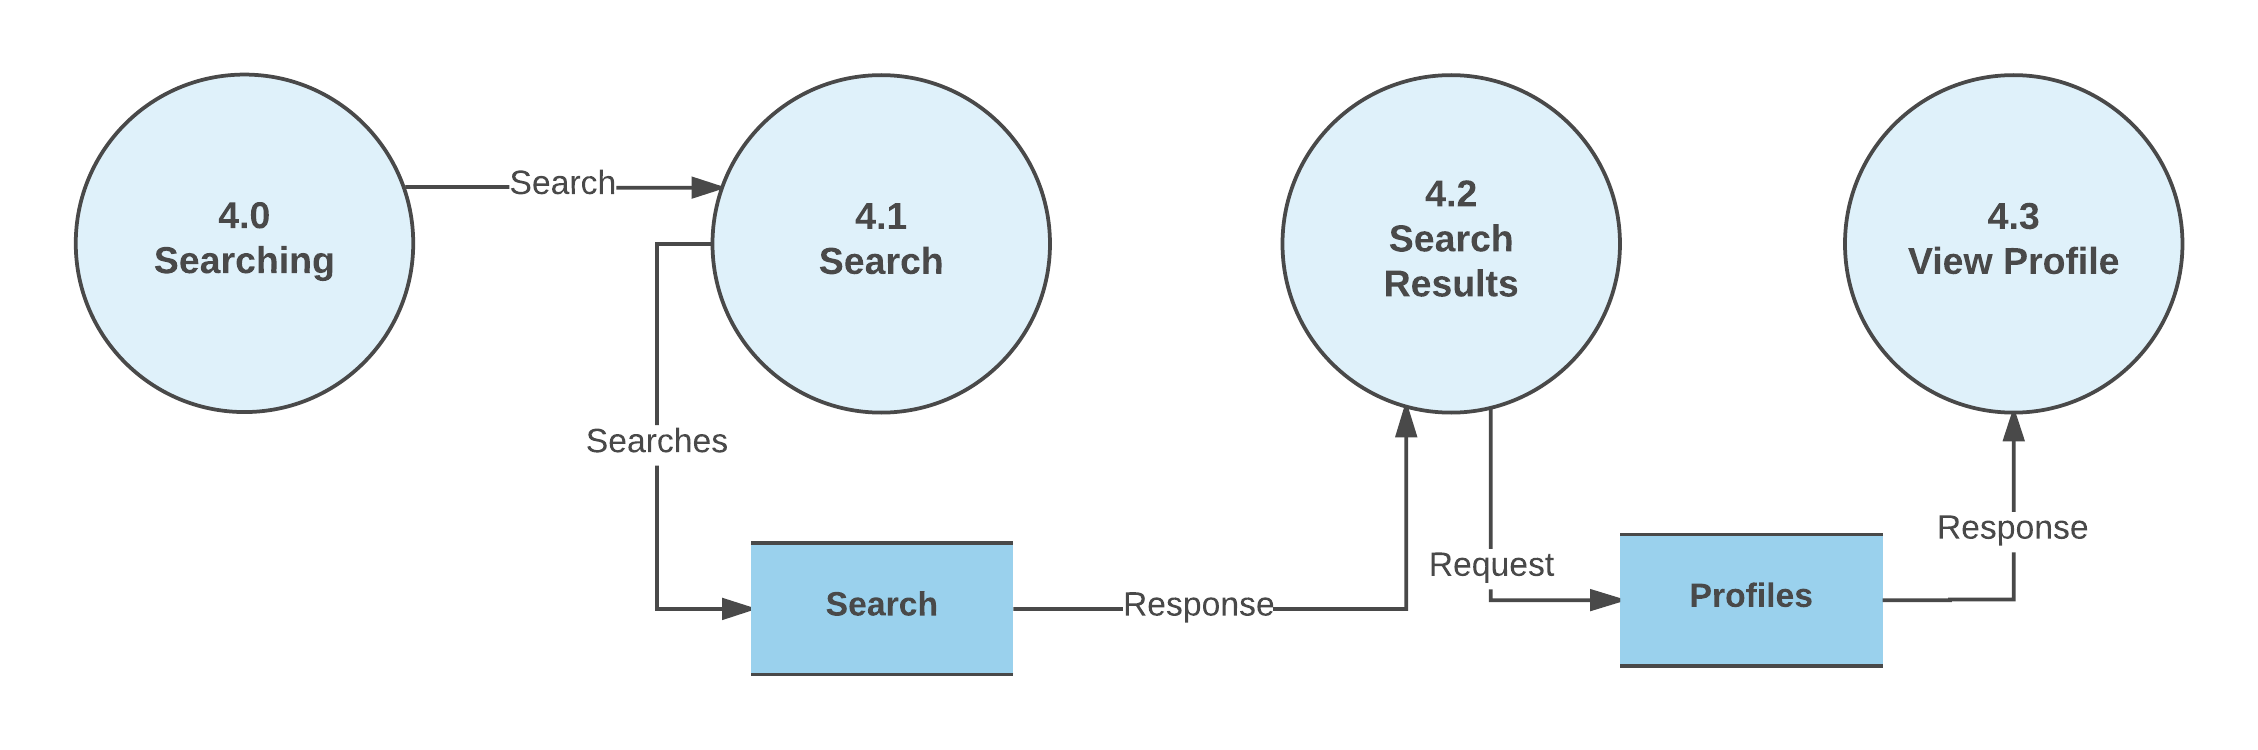
\includegraphics[width=.8\textwidth]{df-l2-4.png}
    \caption{DFD Level 2.4}
    \label{fig:dfd l2.4}
\end{figure}

\begin{figure}[!htb]
    \centering
    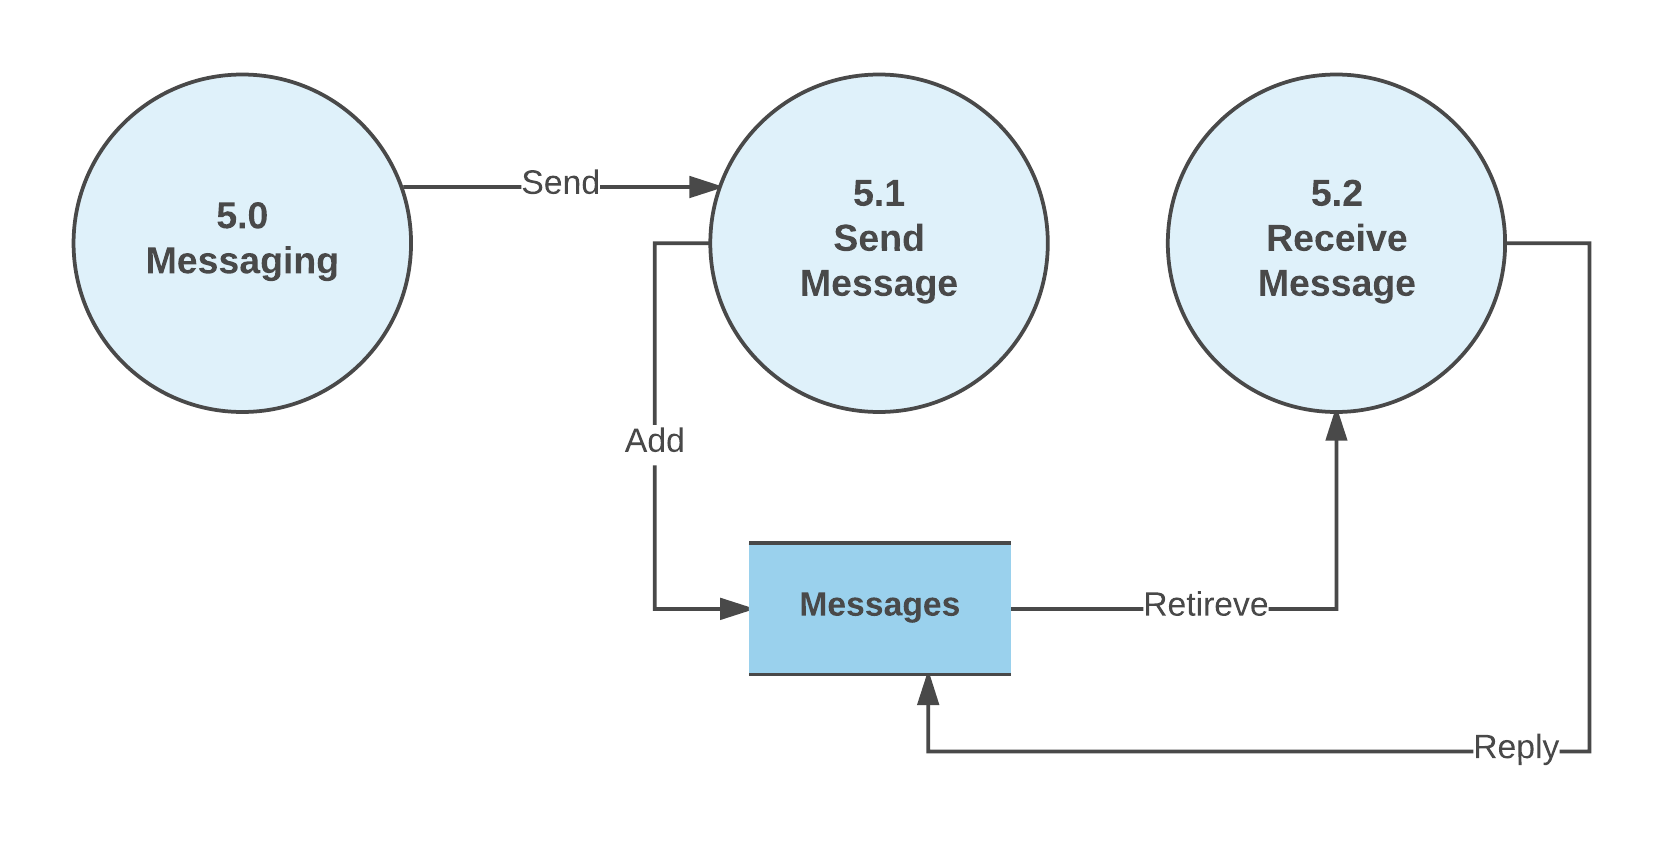
\includegraphics[width=.8\textwidth]{df-l2-5.png}
    \caption{DFD Level 2.5}
    \label{fig:dfd l2.5}
\end{figure}

\begin{figure}[!htb]
    \centering
    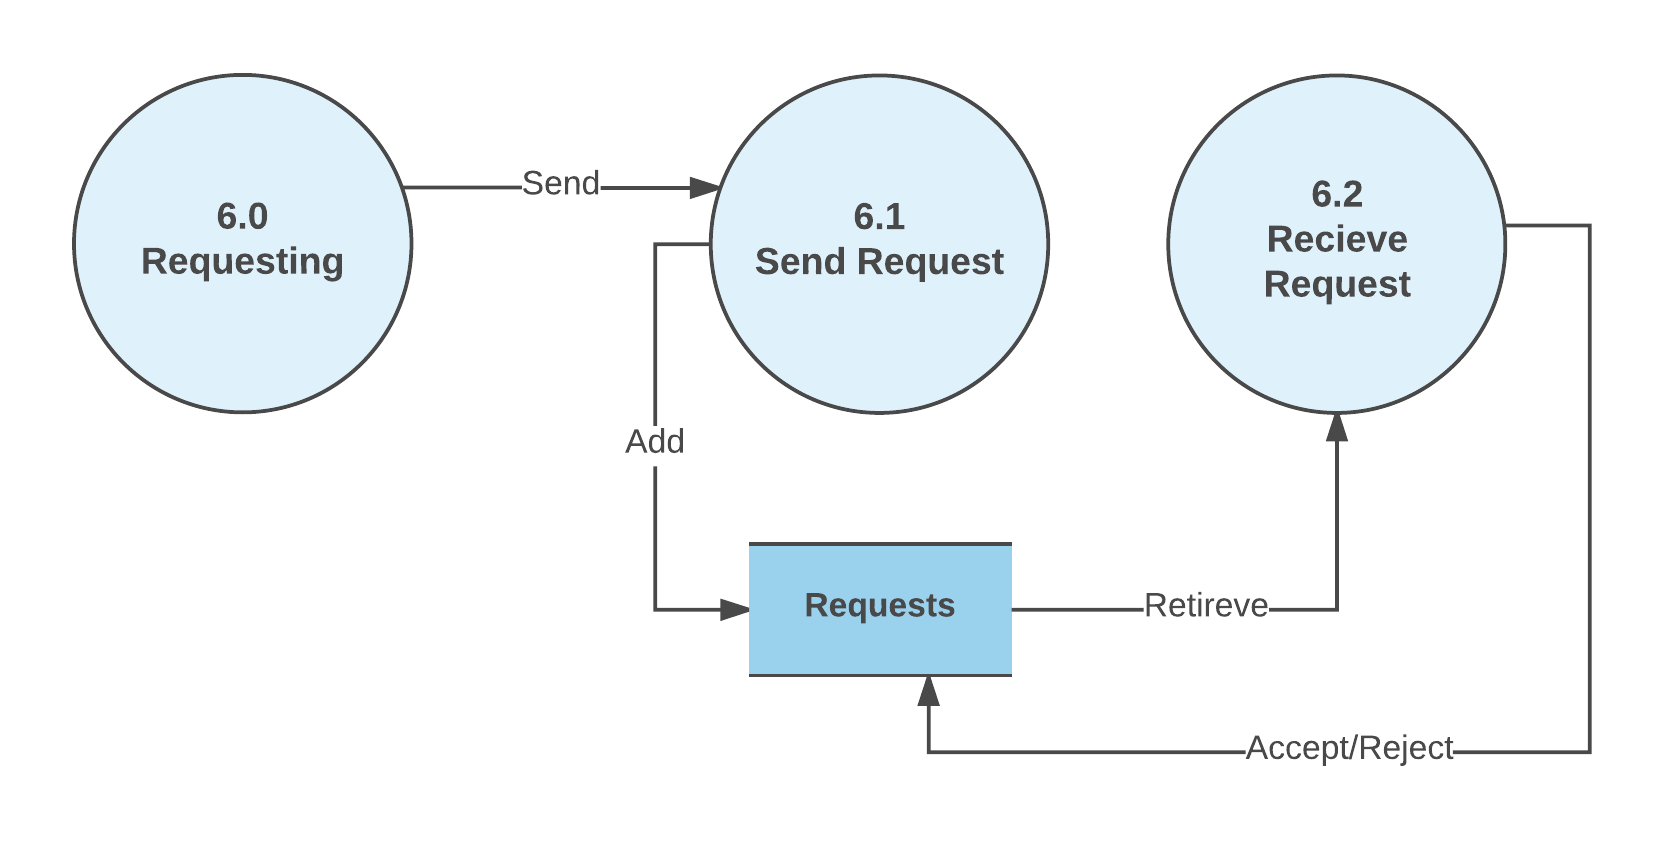
\includegraphics[width=.8\textwidth]{df-l2-6.png}
    \caption{DFD Level 2.6}
    \label{fig:dfd l2.6}
\end{figure}

\begin{figure}[!htb]
    \centering
    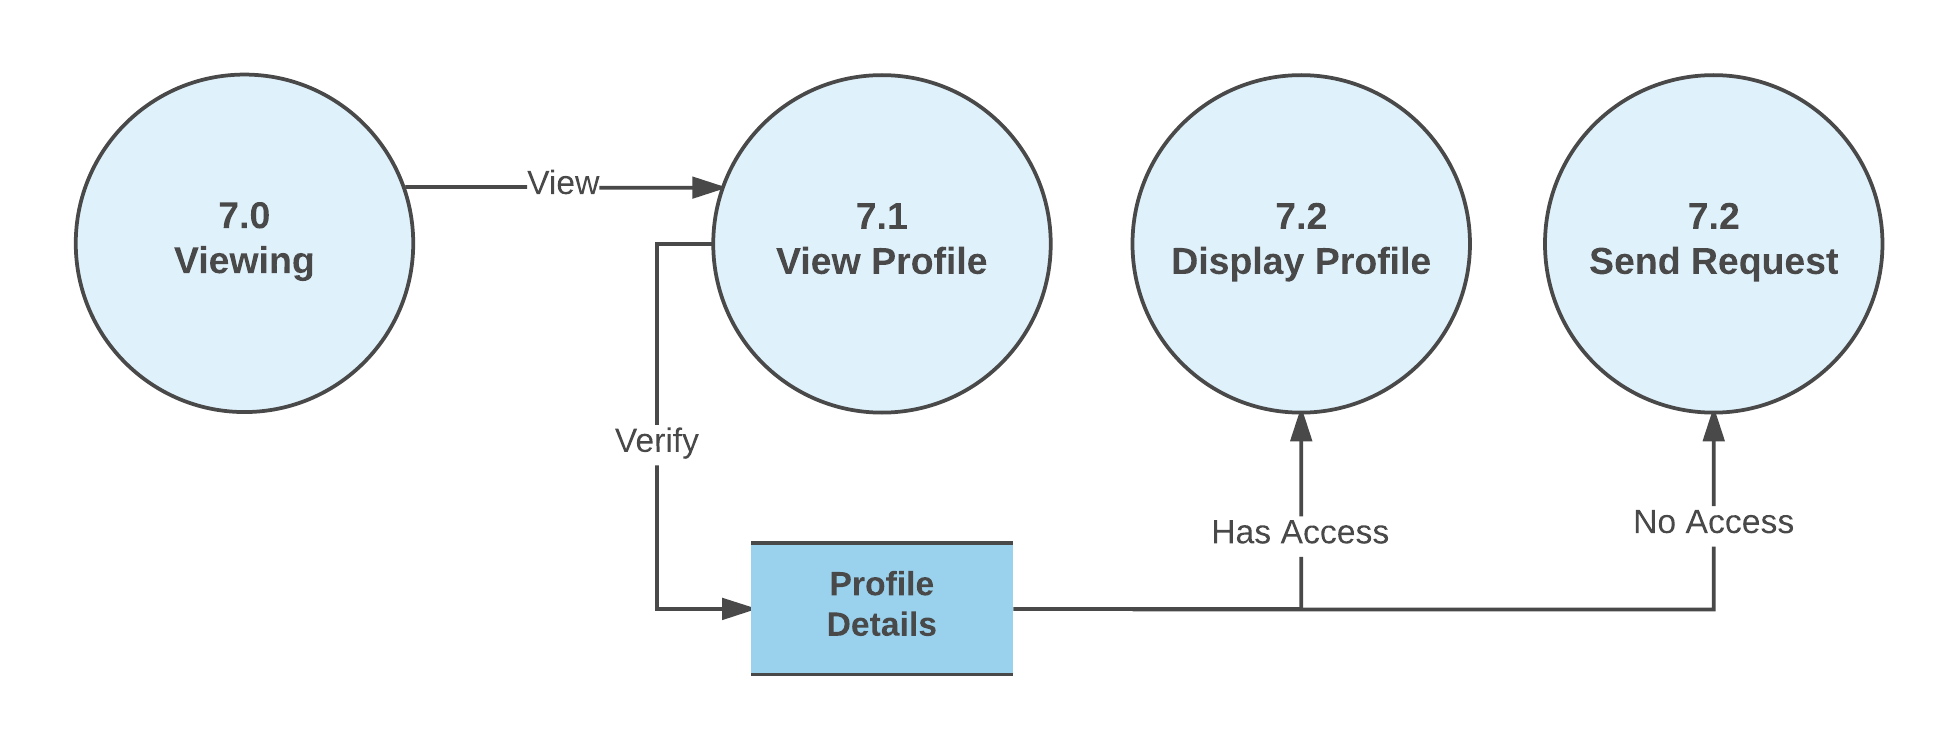
\includegraphics[width=.8\textwidth]{df-l2-7.png}
    \caption{DFD Level 2.7}
    \label{fig:dfd l2.7}
\end{figure}

\begin{figure}[!htb]
    \centering
    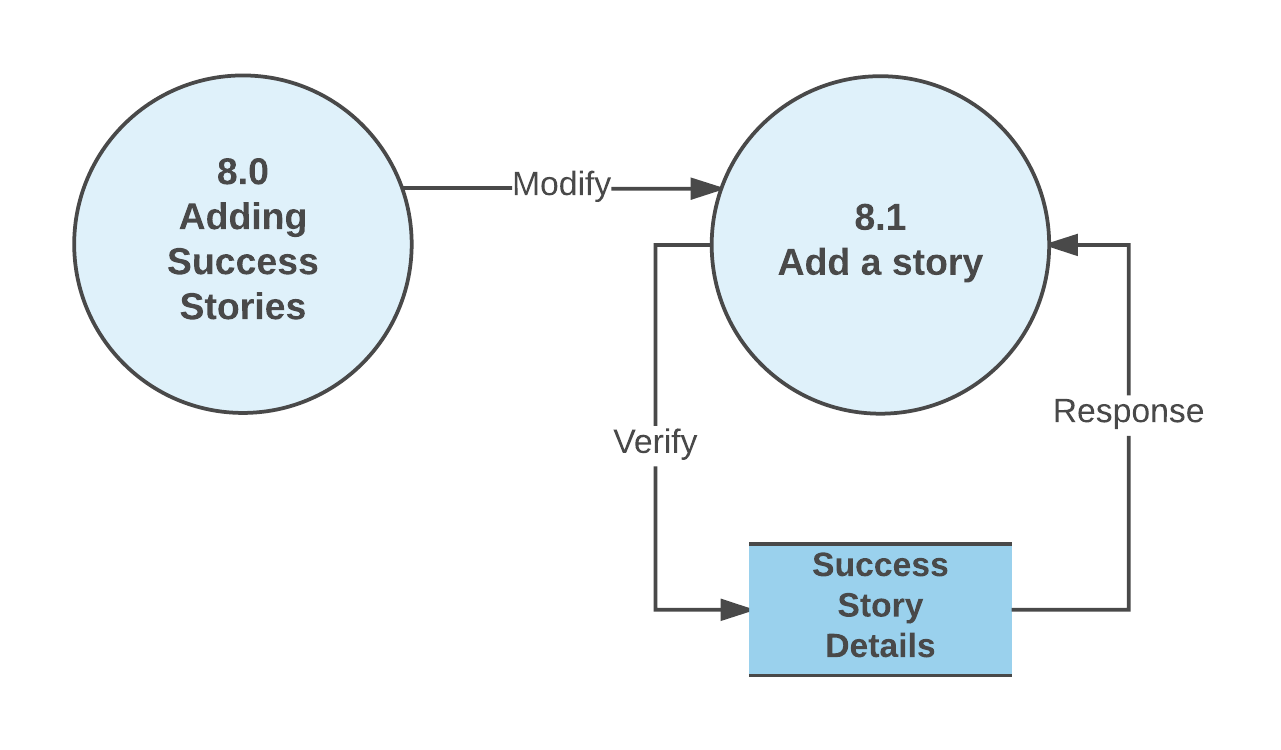
\includegraphics[width=.7\textwidth]{df-l2-8.png}
    \caption{DFD Level 2.8}
    \label{fig:dfd l2.8}
\end{figure}


\chapter{ER Diagram}

\paragraph{}
An entity relationship diagram (ERD) shows the relationships of entity sets stored in a database. An entity in this context is a component of data. In other words, ER diagrams illustrate the logical structure of databases. An entity–relationship model is usually the result of systematic analysis to define and describe what is important to processes in an area of a business. It does not define the business processes; it only presents a business data schema in graphical form. It is usually drawn in a graphical form as boxes (entities) that are connected by lines (relationships) which express the associations and dependencies between entities. \\
 
Entities may be characterized not only by relationships, but also by additional properties (attributes), which include identifiers called "primary keys". Diagrams created to represent attributes as well as entities and relationships may be called entity-attribute-relationship diagrams, rather than entity-relationship models.\\
 
An ER model is typically implemented as a database. In a simple relational database implementation, each row of a table represents one instance of an entity type, and each field in a table represents an attribute type. In a relational database a relationship between entities is implemented by storing the primary key of one entity as a pointer or "foreign key" in the table of another entity.\\

The ER Diagram shown below provides details about the design of the Matrimonial Database system where each entity consists of various non composite attributes that make up a set of prime and non prime attributes. The relationships between the various entities is depicted with the (min ,max) constraints specified. This notation involves associating a pair of integer numbers (min,max) with each participation of an entity type E in a relationship type R, where 0 min less than or equal to max and max greater than or equal to 1 . The numbers mean that for each entity e in E, e must participate in at least min and at most max relationship instances in R at any point of time.  


\begin{figure}[!htb]
    \centering
    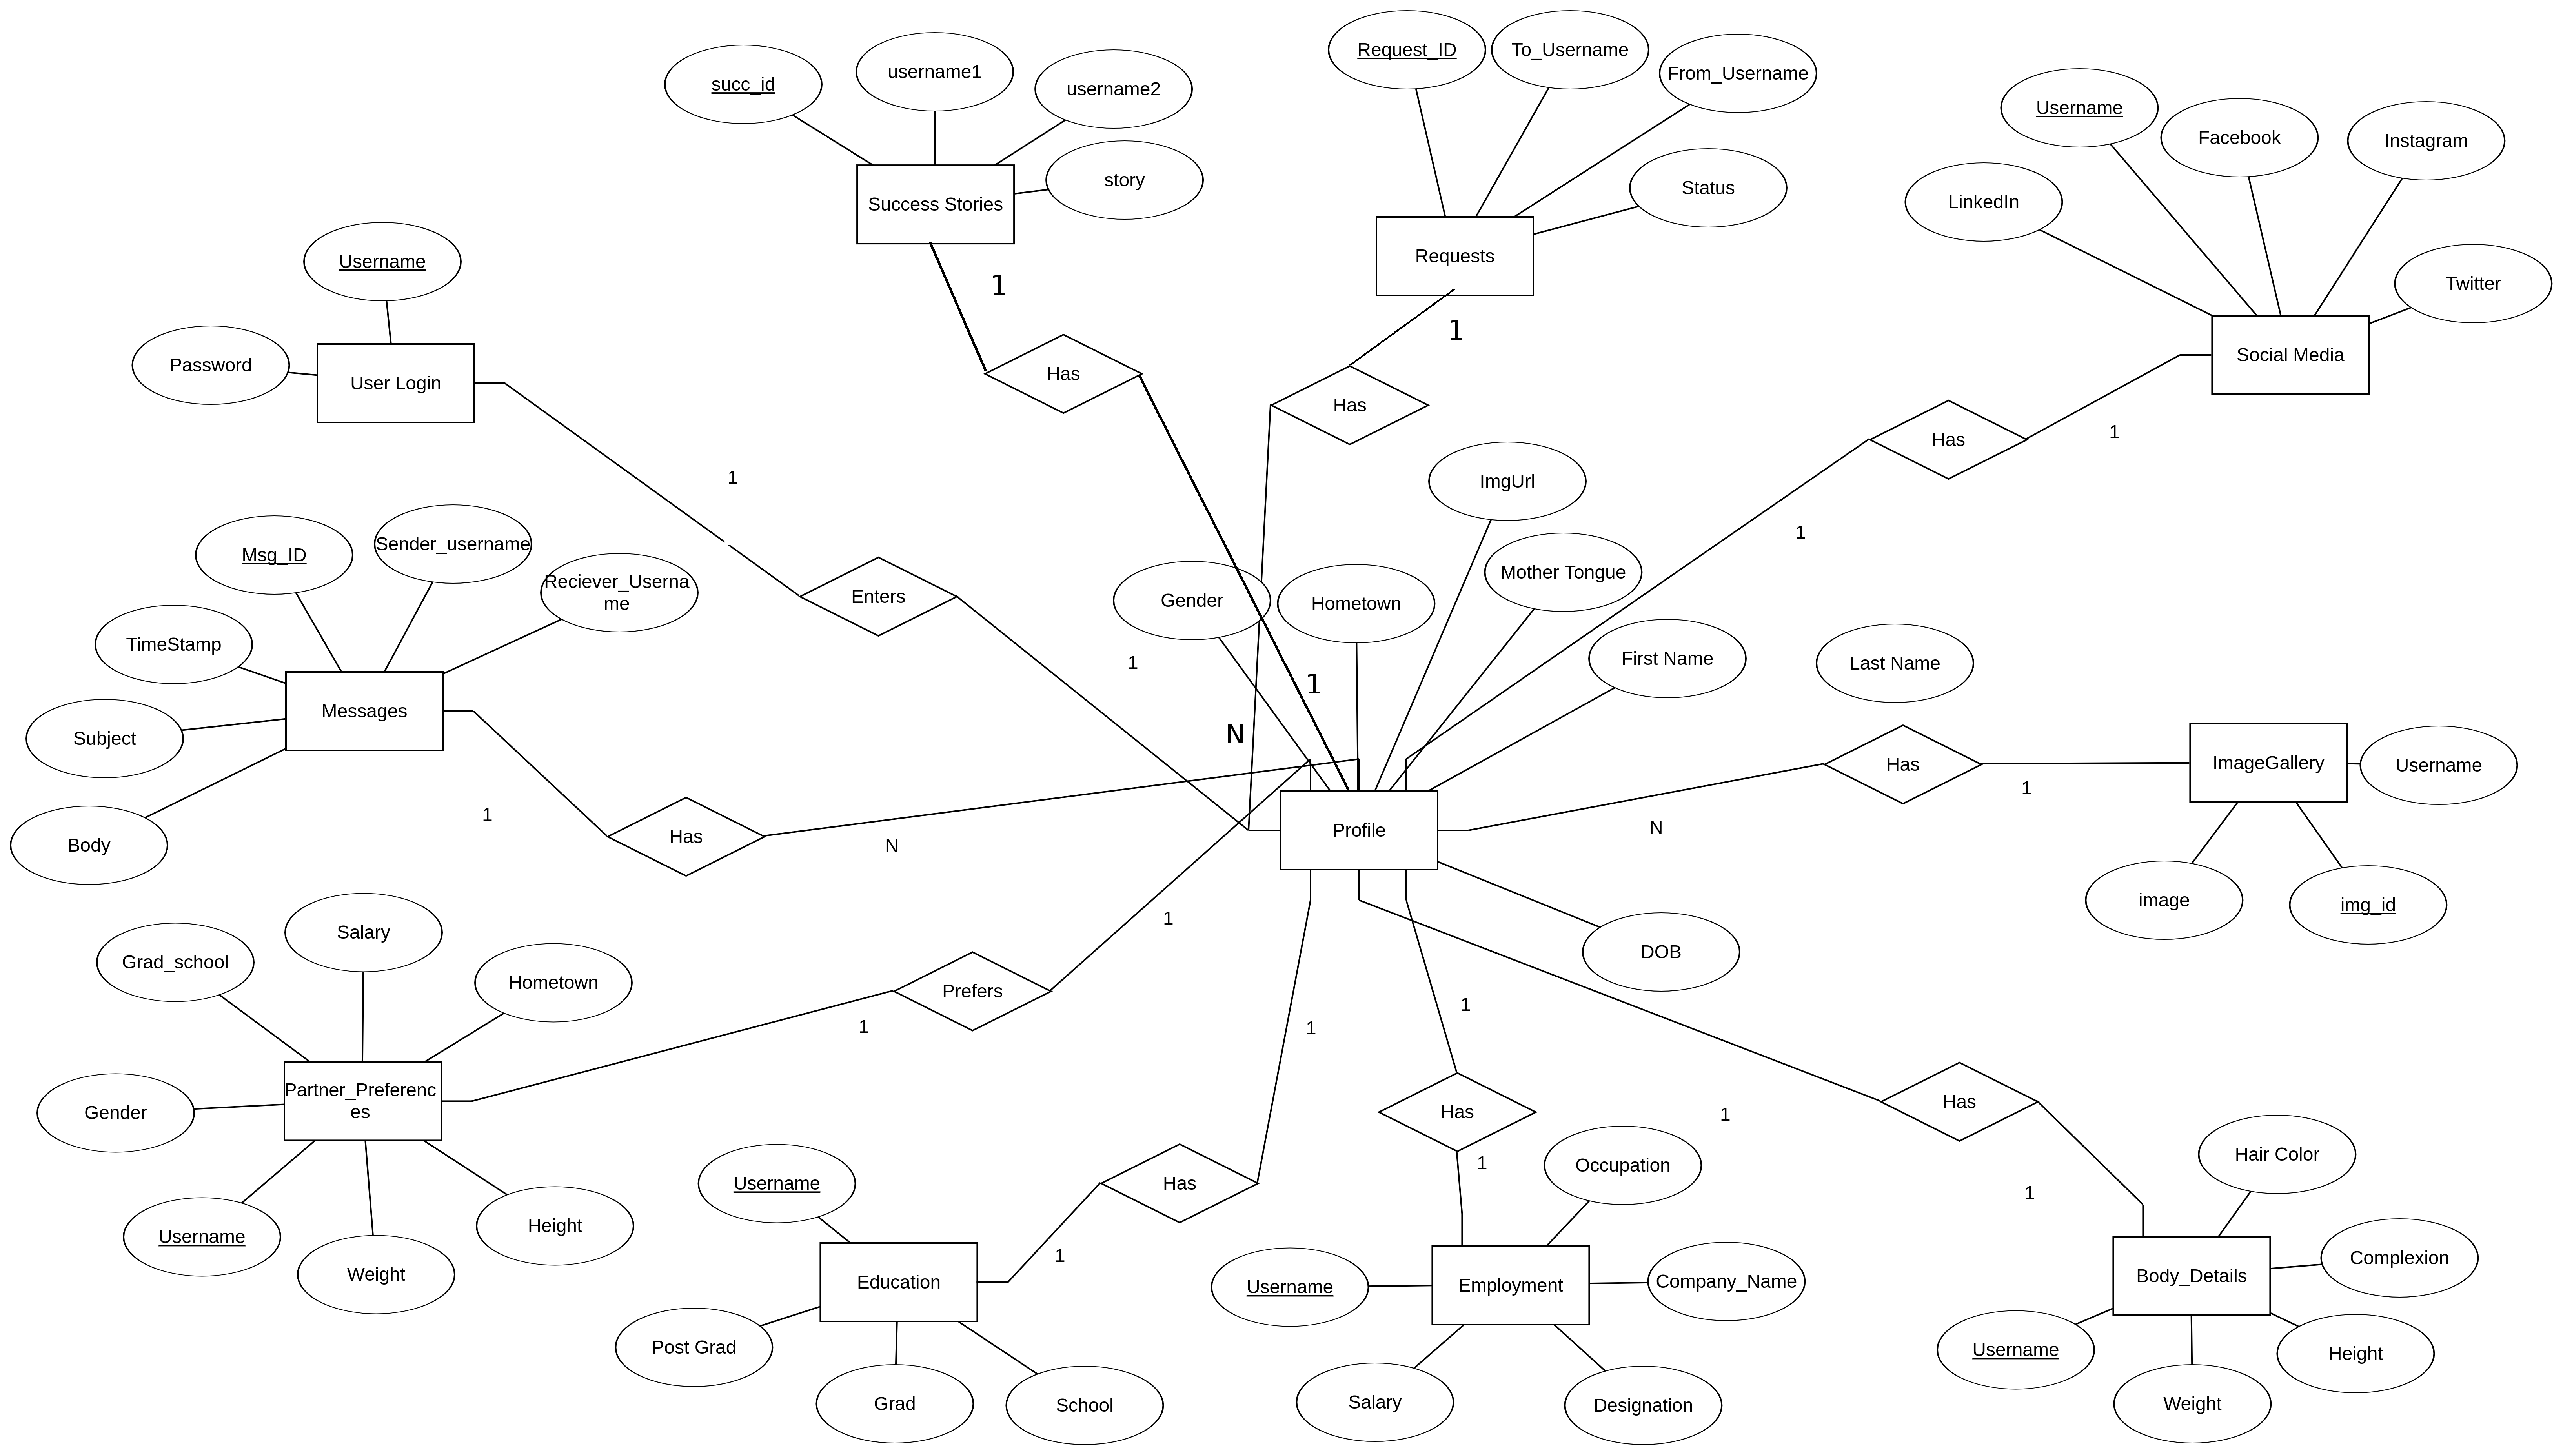
\includegraphics[width=1.3\textwidth, angle = 270]{ER.png}
    \caption{ER Diagram}
    \label{fig:ER Diagram}
\end{figure}





\chapter{Relational Schema and Normalization}
The term \emph{schema} refers to the organization of data as a blueprint of how the database is constructed. The formal definition of a database schema is a set of formulas (sentences) called integrity constraints imposed on a database. Before you can define the database tables using a specific database management software and DDL (Data Definition Language), you must write a relation schema for each table. The set of relation schemas form the relational database schema which is used as input when defining the database.\\

Database normalization, or simply normalization, is the process of organizing the columns (attributes) and tables (relations) of a relational database to reduce data redundancy and improve data integrity. Normalization is also the process of simplifying the design of a database so that it achieves the optimal structure composed of atomic elements. 

\paragraph*{1NF : First Normal Form}
1NF is a property of a relation in a relational database. A relation is in first normal form if and only if the domain of each attribute contains only atomic (indivisible) values, and the value of each attribute contains only a single value from that domain.

\paragraph*{2NF : Second Normal Form}
A relation that is in first normal form (1NF) must meet additional criteria if it is to qualify for second normal form. Specifically: a relation is in 2NF if it is in 1NF and no non-prime attribute is dependent on any proper subset of any candidate key of the relation. A non-prime attribute of a relation is an attribute that is not a part of any candidate key of the relation. \\
Put simply, a relation is in 2NF if it is in 1NF and every non-prime attribute of the relation is dependent on the whole of every candidate key.

\paragraph*{3NF : Third Normal Form}
Codd's definition states that a table is in 3NF if and only if both of the following conditions hold:-
\begin{itemize}
\item The relation R (table) is in second normal form (2NF)
\item Every non-prime attribute of R is non-transitively dependent on every key of R.
\end{itemize}

\noindent Every non-prime attribute of R is non-transitively dependent on every key of R.
A non-prime attribute of R is an attribute that does not belong to any candidate key of R.\\
 A transitive dependency is a functional dependency in which 
 $ X \rightarrow Z $ (X determines Z) indirectly, by virtue of $X \rightarrow Y$ and $Y \rightarrow Z$ (where it is not the case that $Y \rightarrow X$). \\\\
 
\noindent The normalized tables of our database is given in the figure below. \\

\noindent The tables are in 1NF since the domain of each attribute contains only atomic (indivisible) values, and the value of each attribute contains only a single value from that domain. \\

\noindent The tables are in 2NF since it is in 1NF and every non-prime attribute of the relation is dependent on the whole of every candidate key. In our tables the candidate keys are the same as the primary keys which is just one attribute in every simple. Therefore this constraint is satisfied. \\
 
\noindent The tables are in 3NF since in it in 2NF and every non-prime attribute of every relation is non-transitively dependent on every key of the relation. There are no inherent transitive dependencies in our relations. \\
 
 
\begin{figure}[!htb]
    \centering
    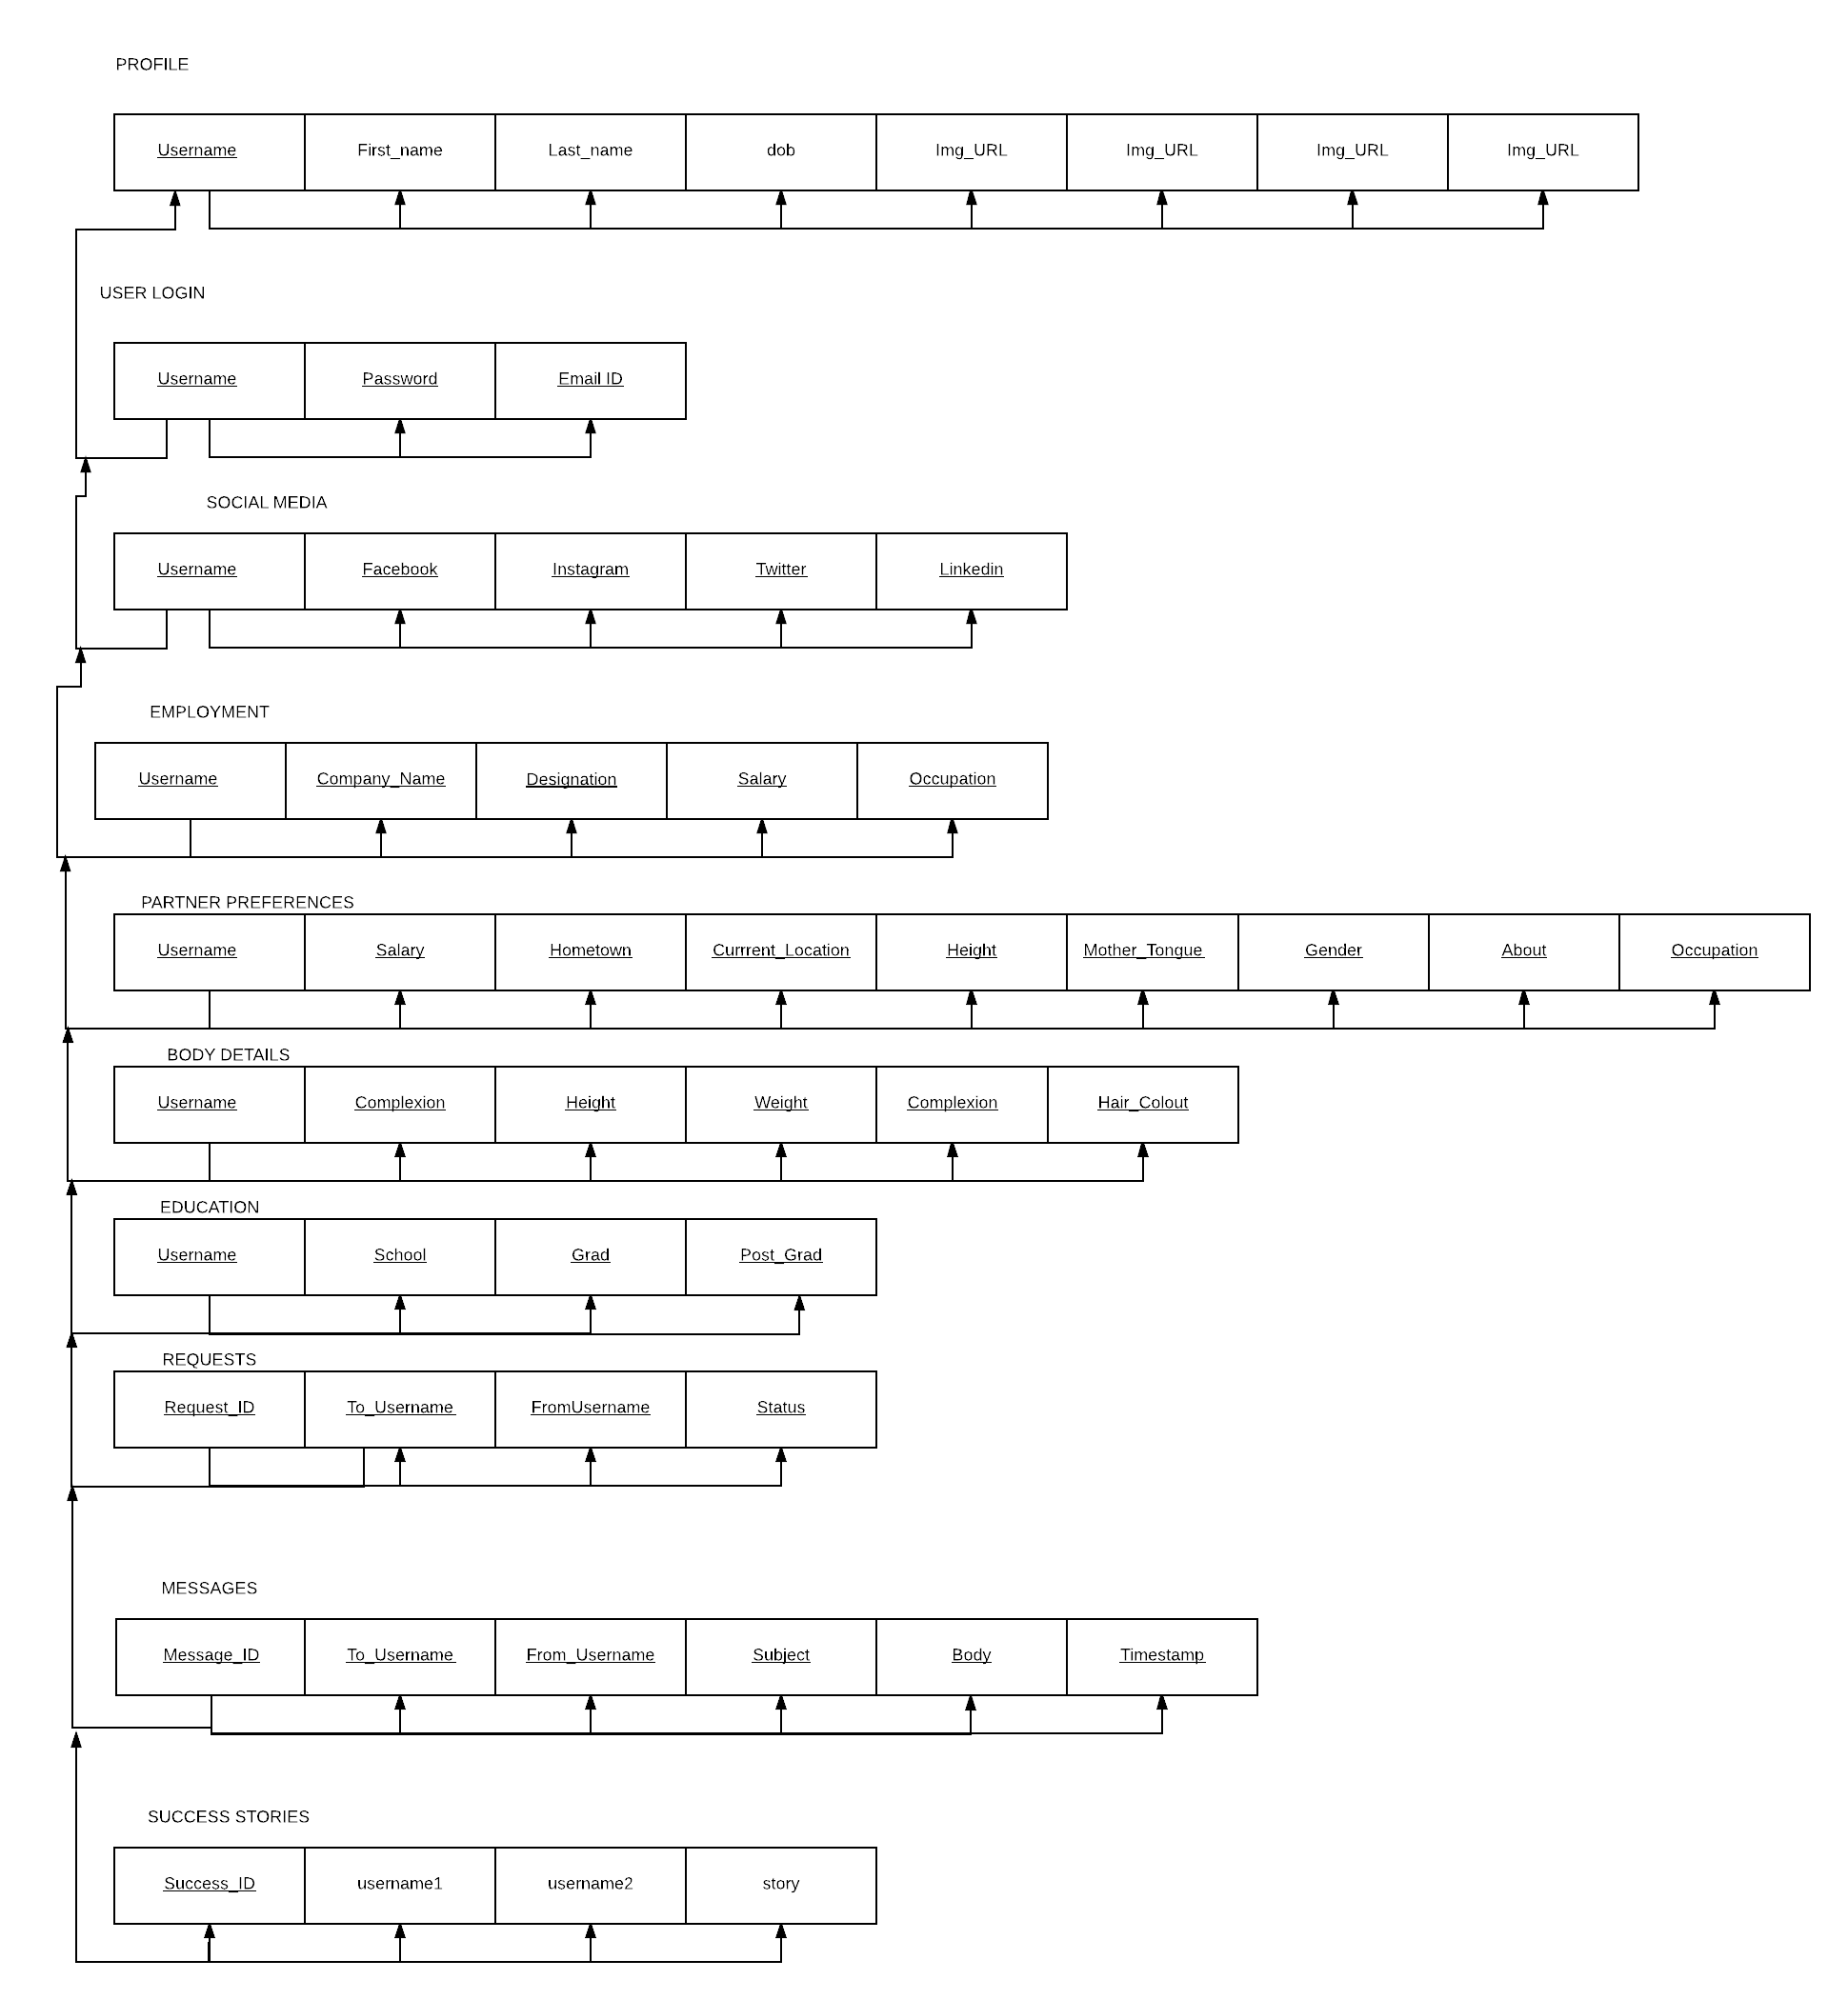
\includegraphics[width=1\textwidth]{Normalized-Tables.png}
    \caption{Normalized Schema}
    \label{fig:Normalized Schema}
\end{figure}
 
\chapter{Reports} 
Most database management systems include a report
writer that enables you to design and generate reports. The process of report generation includes
collecting suitable data from multiple functionalities and displaying to the end user. A report usually
summarizes the entire functionality of the database management system that is design. \\\\
Users can click on the Generate Bio button to generate a download-able PDF of their profile. This PDF will contain all the information that they have entered in their profile. \\\\
Given below is an example of the report generated for a particular user.

\begin{figure}[!htb]
    \centering
    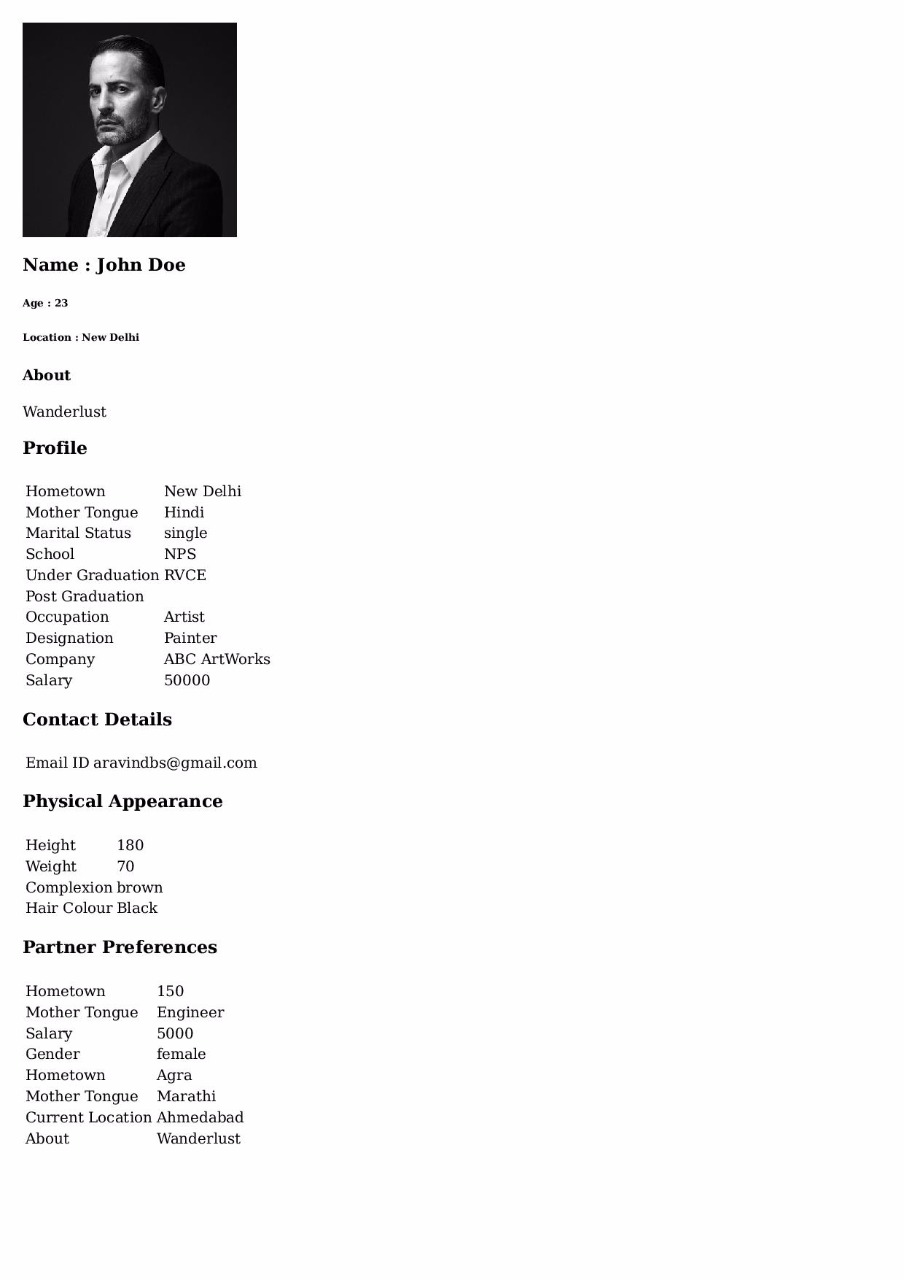
\includegraphics[width=.9\textwidth]{report.jpeg}
    \caption{Report}
    \label{fig:Report}
\end{figure} 

\chapter{Conclusions}
\section{Summary}
\paragraph*{•}
 
 The matrimonial site developed allows one to explore various matchmaking opportunities to find a viable or suitable partner whom he/she feels truly connected to.\\

The site promotes socializing and offers numerous possibilities by allowing users to sift through the sea of humanity that we normally face in an organized and easy manner.The implementation of an user friendly interface will indubitably makes the premise of background checks easier as documents such as ID proofs necessary for verification can be uploaded seamlessly using a one-click.\\


Furthermore, the messaging service developed and request access can help dispel several myths and fancies and allow a free and uninhibited social sphere which in turn may often lead to promising matchmaking.


\section{Limitations}
\paragraph*{•}
 
\begin{enumerate}
\item Users cannot set different levels of privacy to different sets of details entered by them. 
\item Users cannot delete the pictures they have uploaded once in the gallery. 
\item Other family members cannot make profiles for their relatives.
\end{enumerate}


\section{Future Enhancements}
\paragraph*{•}
 
\begin{enumerate}
\item Automatic recommendations of user profiles using a sophisticated matching algorithm.  
\item Implementation of live chat with multiple users.
\item Varying levels of privacy for different sets of details.
\item Multiple types of users, for example as a mother or father.
\item Multiple types of users, for example those who have a Premium Membership. 

\end{enumerate}

\chapter{References} 


\noindent [1] Roger S Presman, 2002. Software Engineering Concepts: A Modern Approach, Prentice Hall, Second Edition. \\\

\noindent [2] Rajib Mall, 2002. Fundamentals of Software Engineering, Prentice Hall, Fifth Edition. \\\

\noindent [3] Elmasri and Navathe,2005. Fundamentals of Database Systems, Pearson, Fifth Edition \\



\noindent [4] https://www.w3schools.com/w3css/default.asp \\\\
\noindent [5] http://jinja.pocoo.org/docs/2.9/templates/\\\\
\noindent [6] https://docs.python.org/2/library/hashlib.html \\\\
\noindent [7] https://realpython.com/blog/python/introduction-to- flask-part- 2-creating- a-login-
page/ \\\\
\noindent [8] https://pypi.python.org/pypi/MySQL-python


\chapter{Appendix: Snapshots} 

\begin{figure}[!htb]
    \centering
    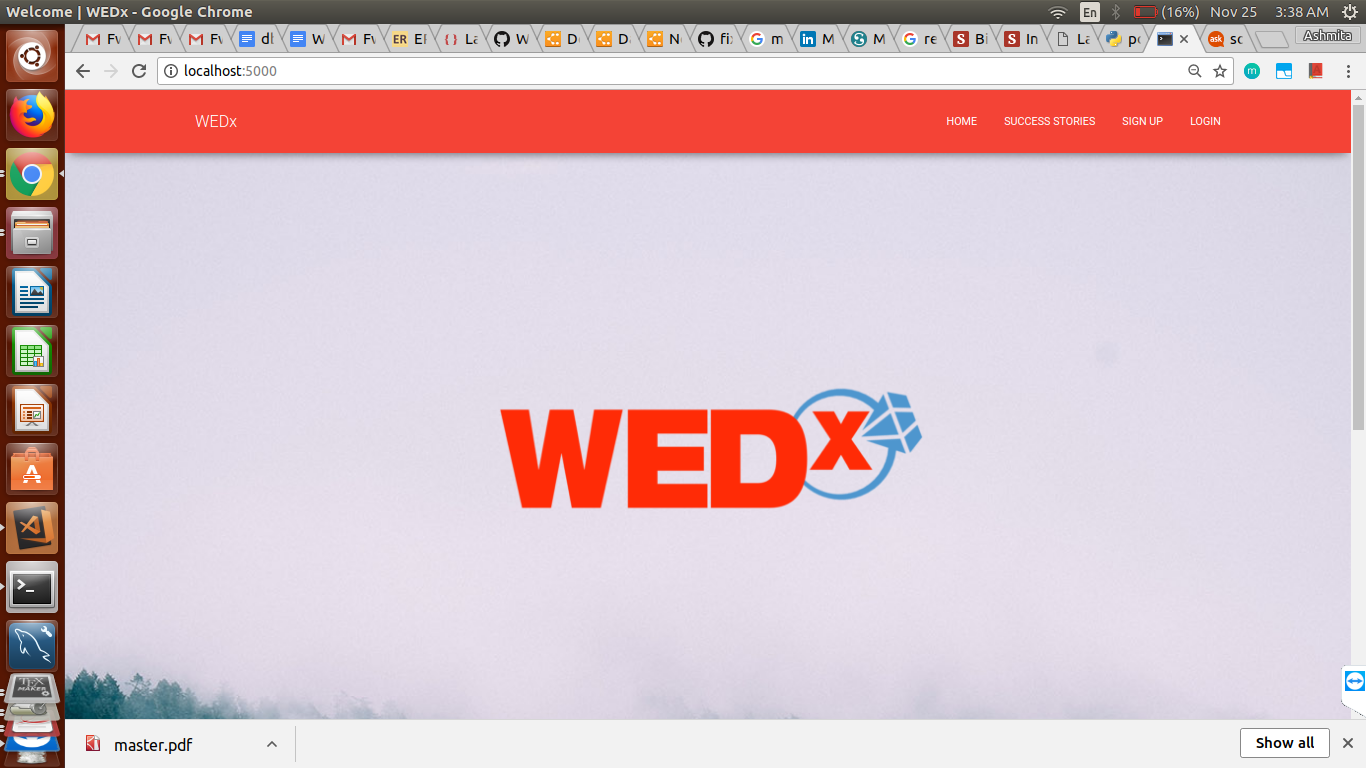
\includegraphics[width=1\textwidth]{sc-1.png}
    \caption{Homepage}
    \label{fig:Homepage}
\end{figure}

\begin{figure}[!htb]
    \centering
    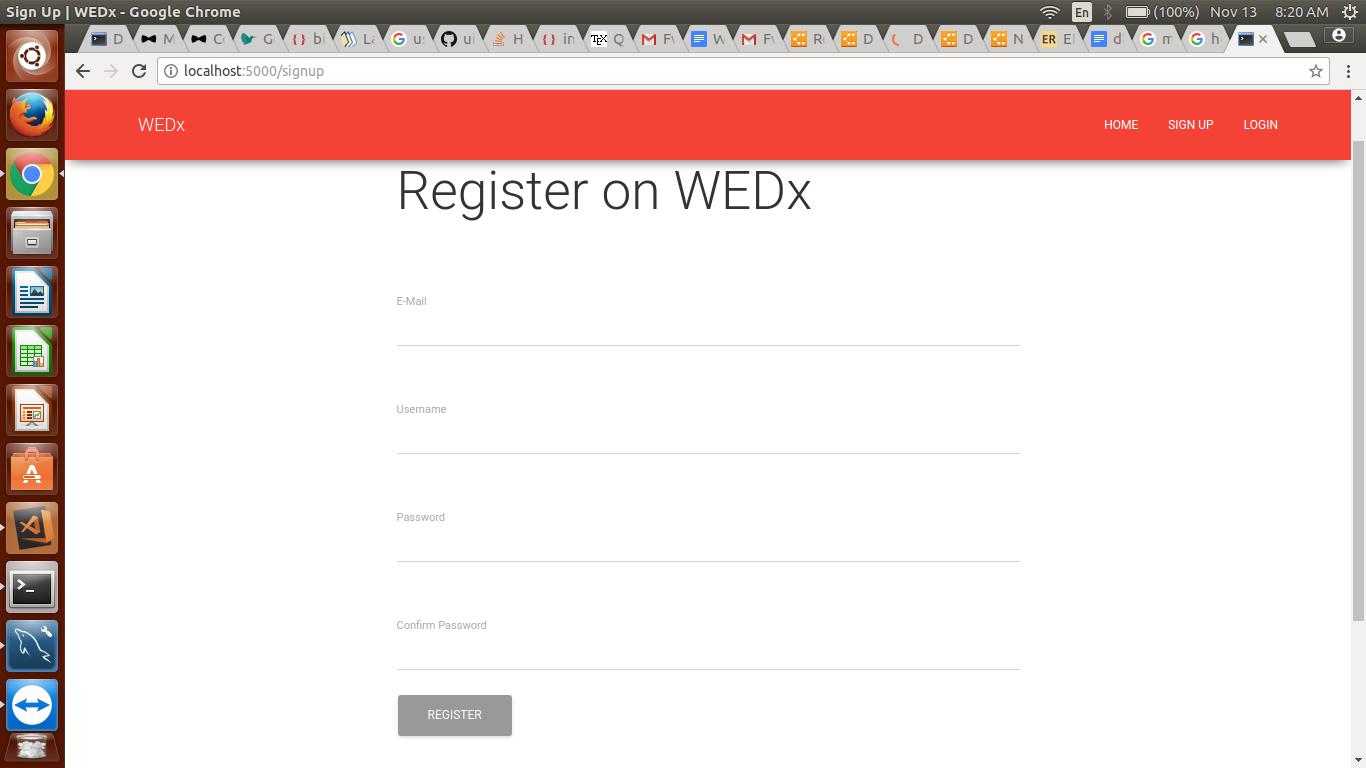
\includegraphics[width=1\textwidth]{sc-2.png}
    \caption{Registration Page}
    \label{fig:Registration Page}
\end{figure}


\begin{figure}[!htb]
    \centering
    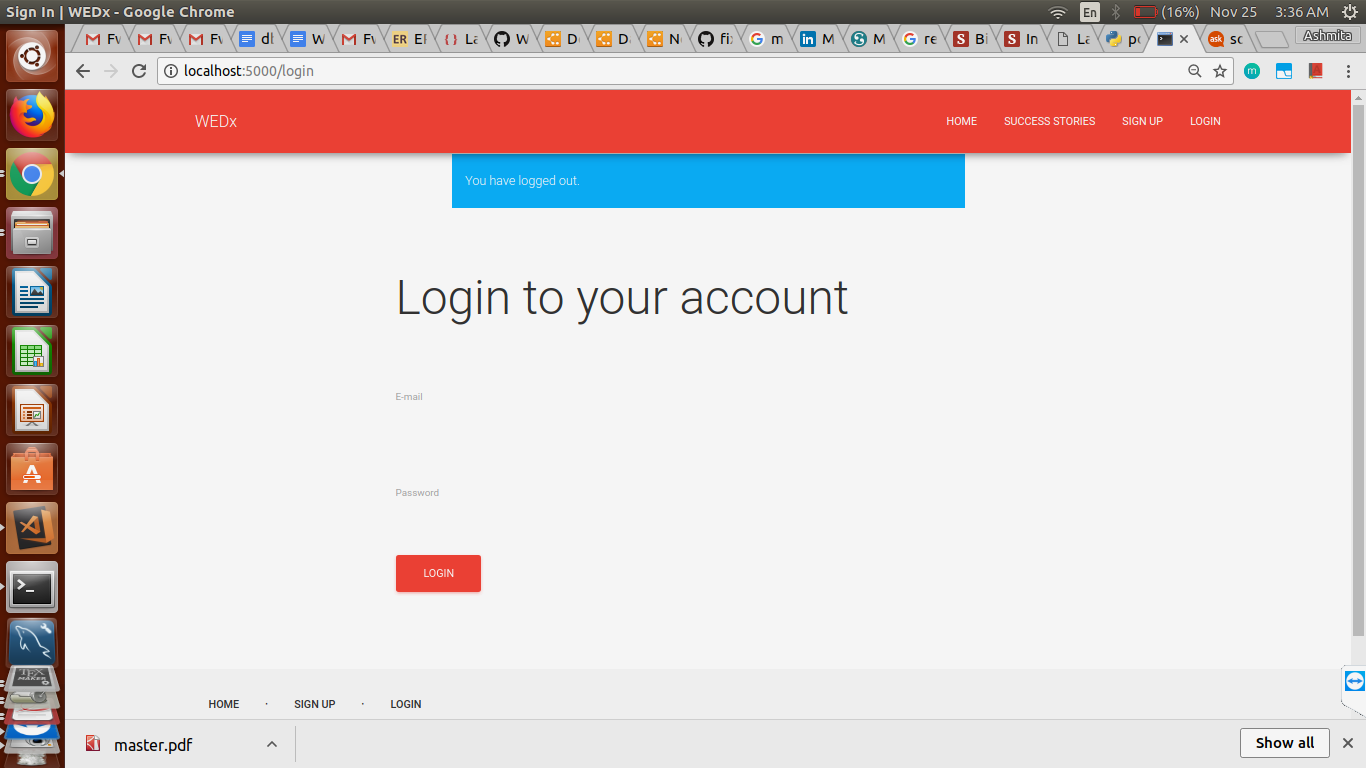
\includegraphics[width=1\textwidth]{sc-25.png}
    \caption{Login Page}
    \label{fig:Login Page}
\end{figure}


\begin{figure}[!htb]
    \centering
    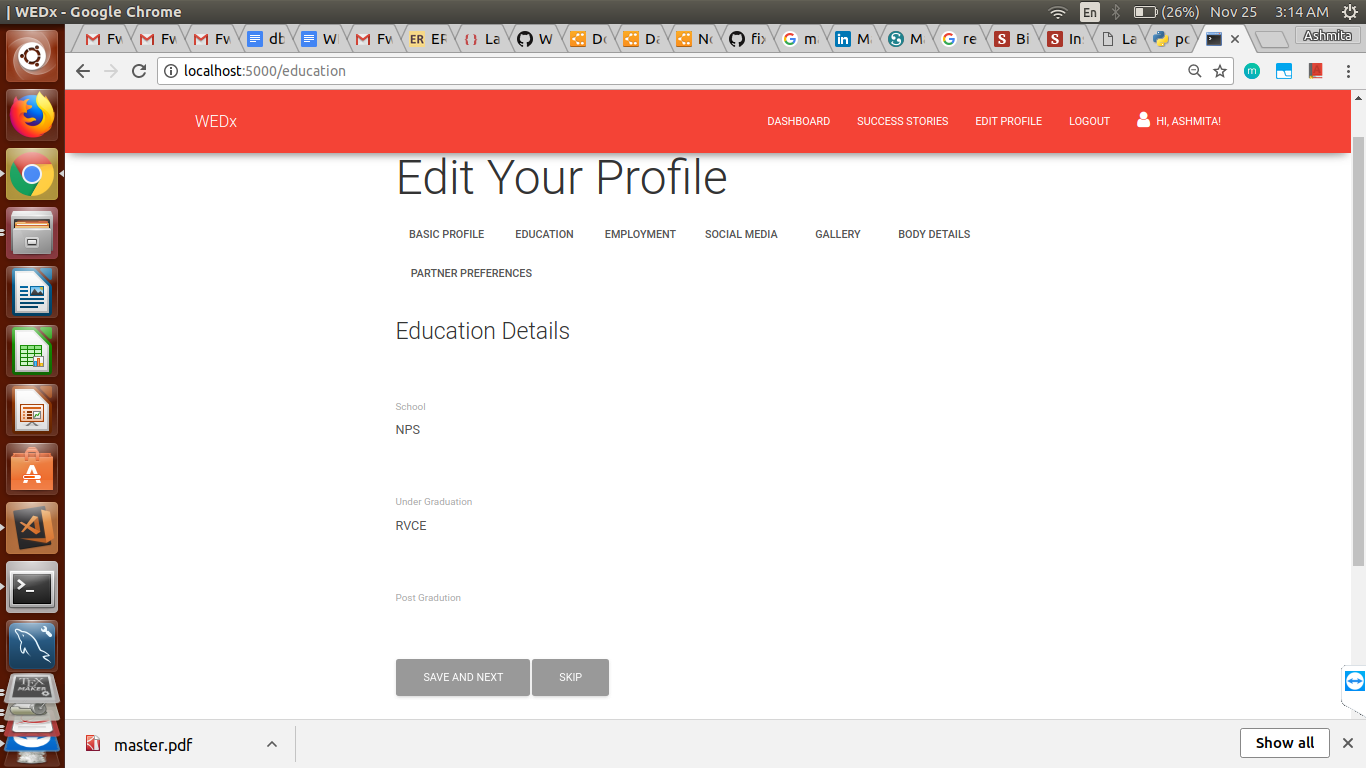
\includegraphics[width=1\textwidth]{sc-3.png}
    \caption{Edit Profile}
    \label{fig:Edit Profile}
\end{figure}

\begin{figure}[!htb]
    \centering
    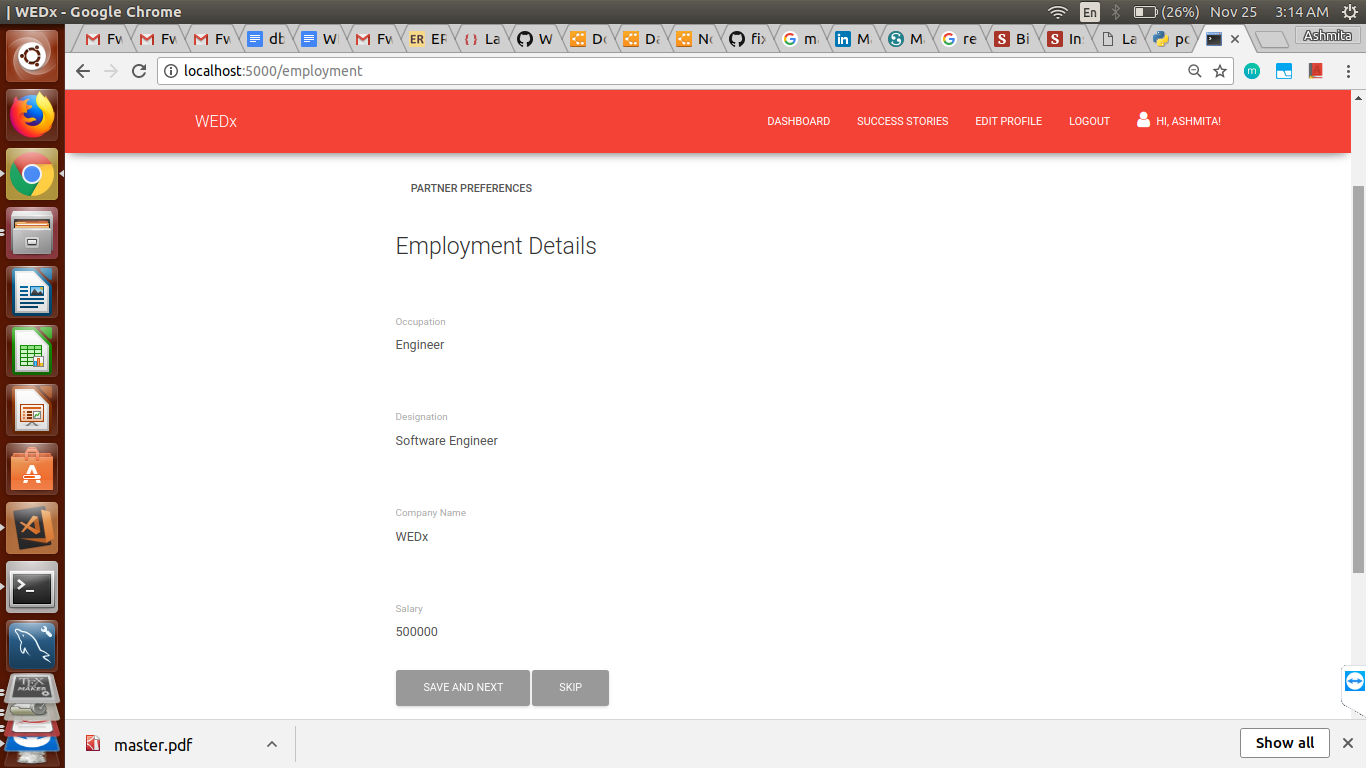
\includegraphics[width=1\textwidth]{sc-4.png}
    \caption{Edit Employment}
    \label{fig:Edit Employment}
\end{figure}

\begin{figure}[!htb]
    \centering
    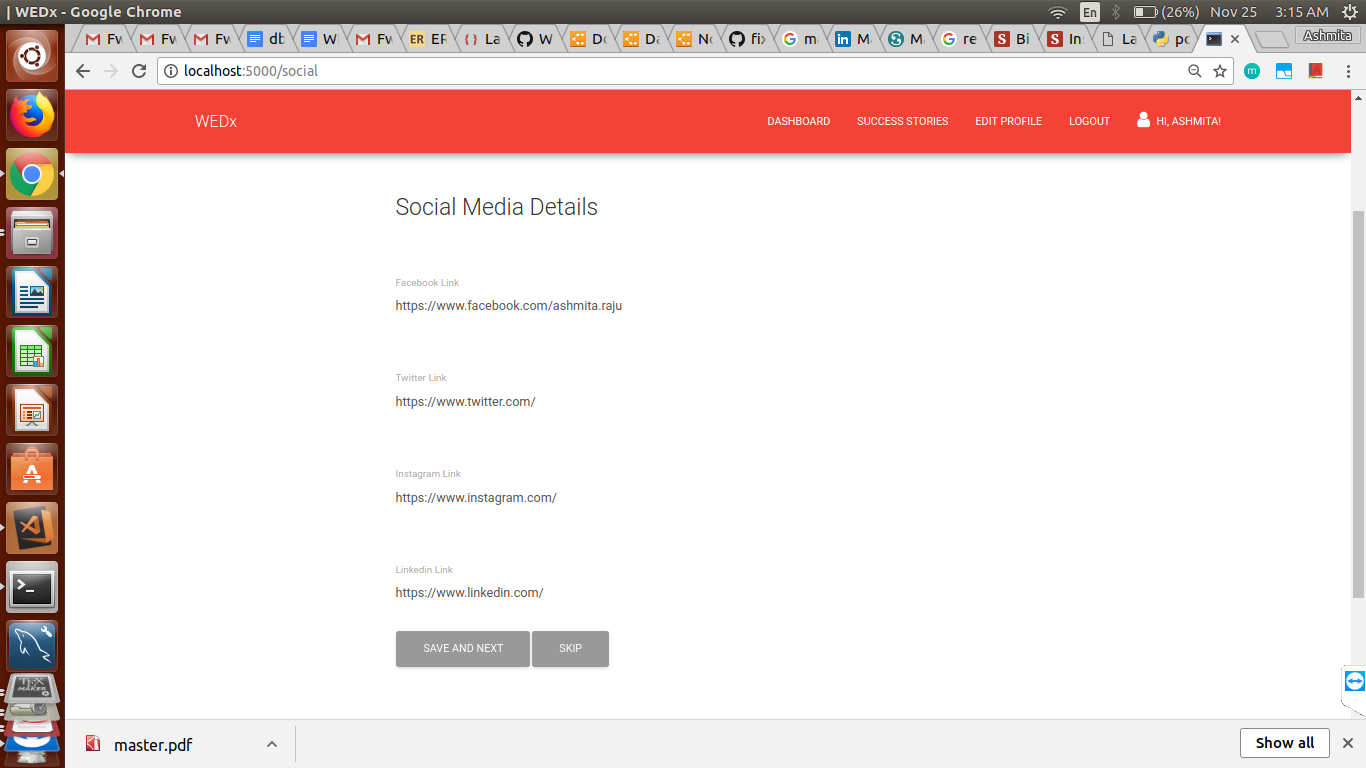
\includegraphics[width=1\textwidth]{sc-5.png}
    \caption{Edit Social Media}
    \label{fig:Edit Social Media}
\end{figure}

\begin{figure}[!htb]
    \centering
    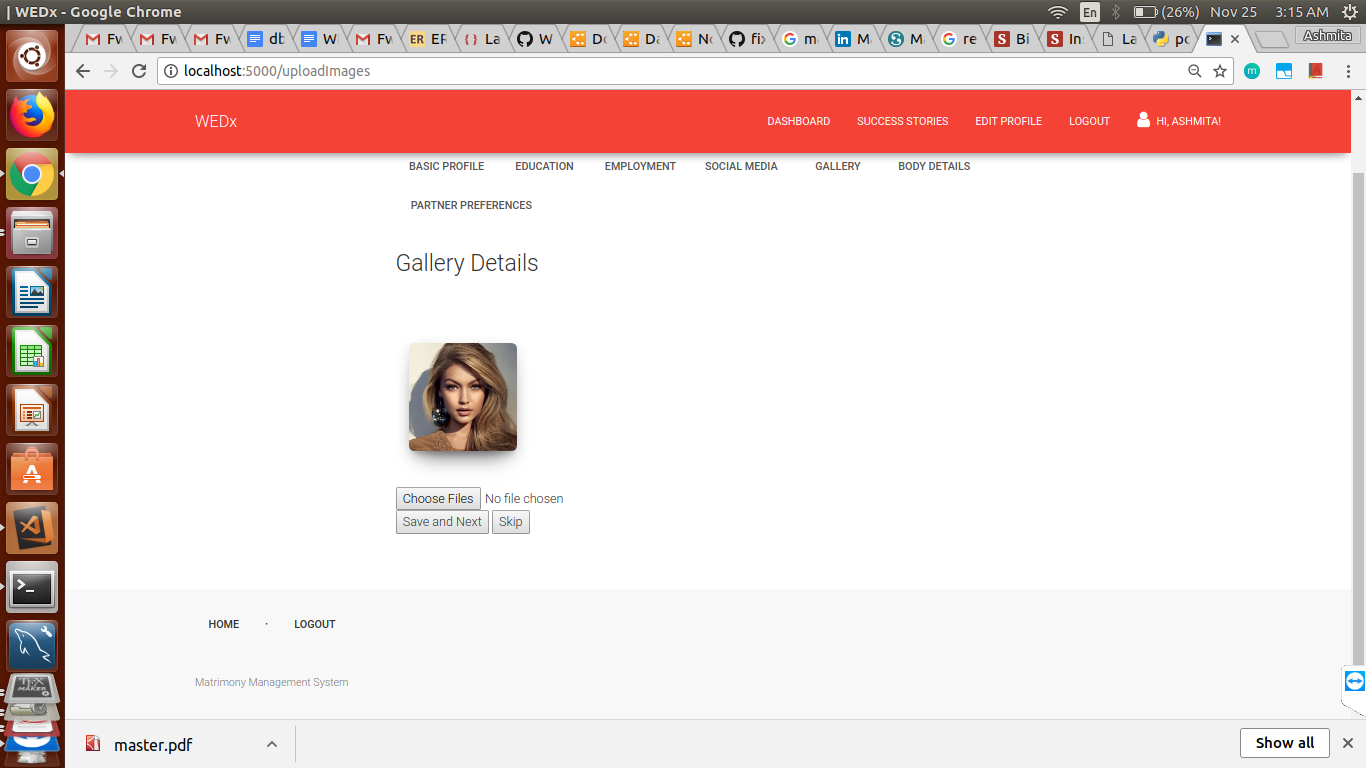
\includegraphics[width=1\textwidth]{sc-6.png}
    \caption{Edit Gallery}
    \label{fig:Edit Gallery}
\end{figure}

\begin{figure}[!htb]
    \centering
    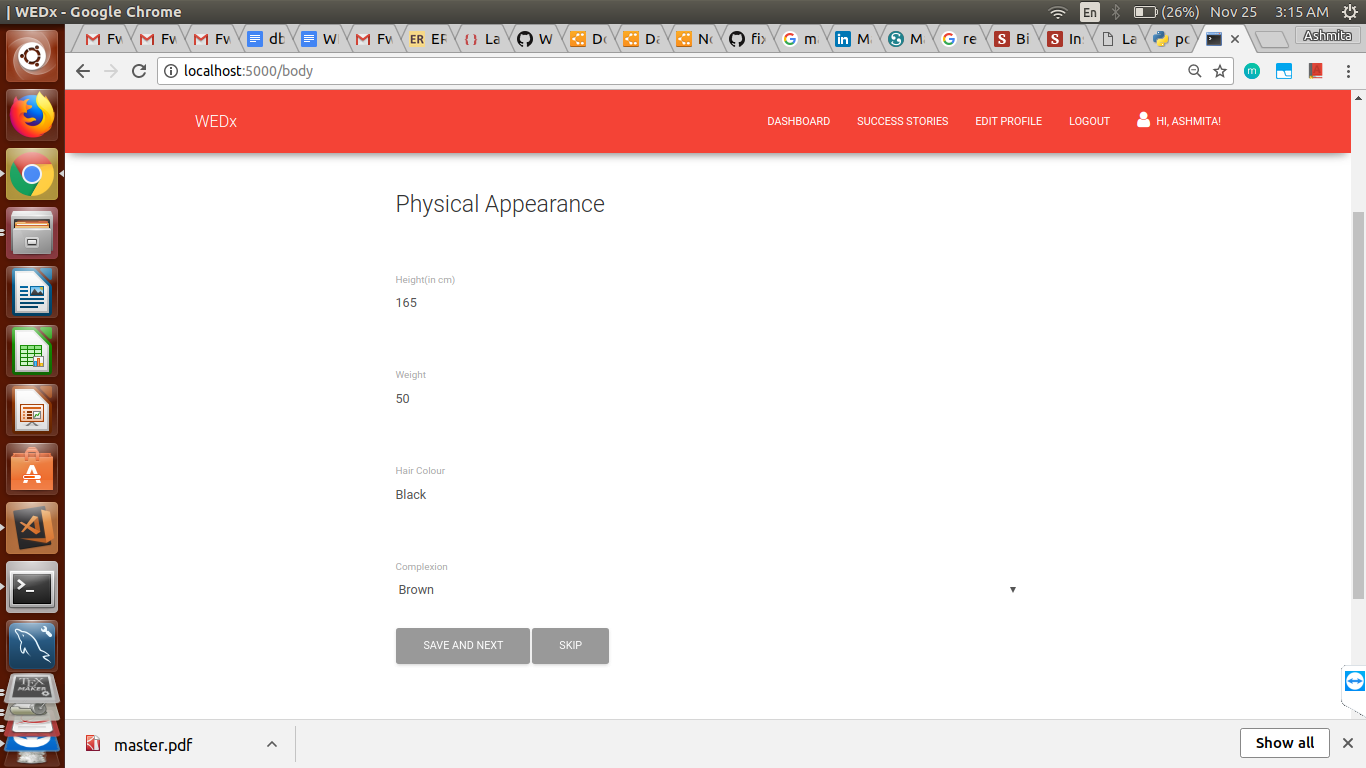
\includegraphics[width=1\textwidth]{sc-7.png}
    \caption{Edit Physical Appearance}
    \label{fig:Edit Physical Appearance}
\end{figure}

\begin{figure}[!htb]
    \centering
    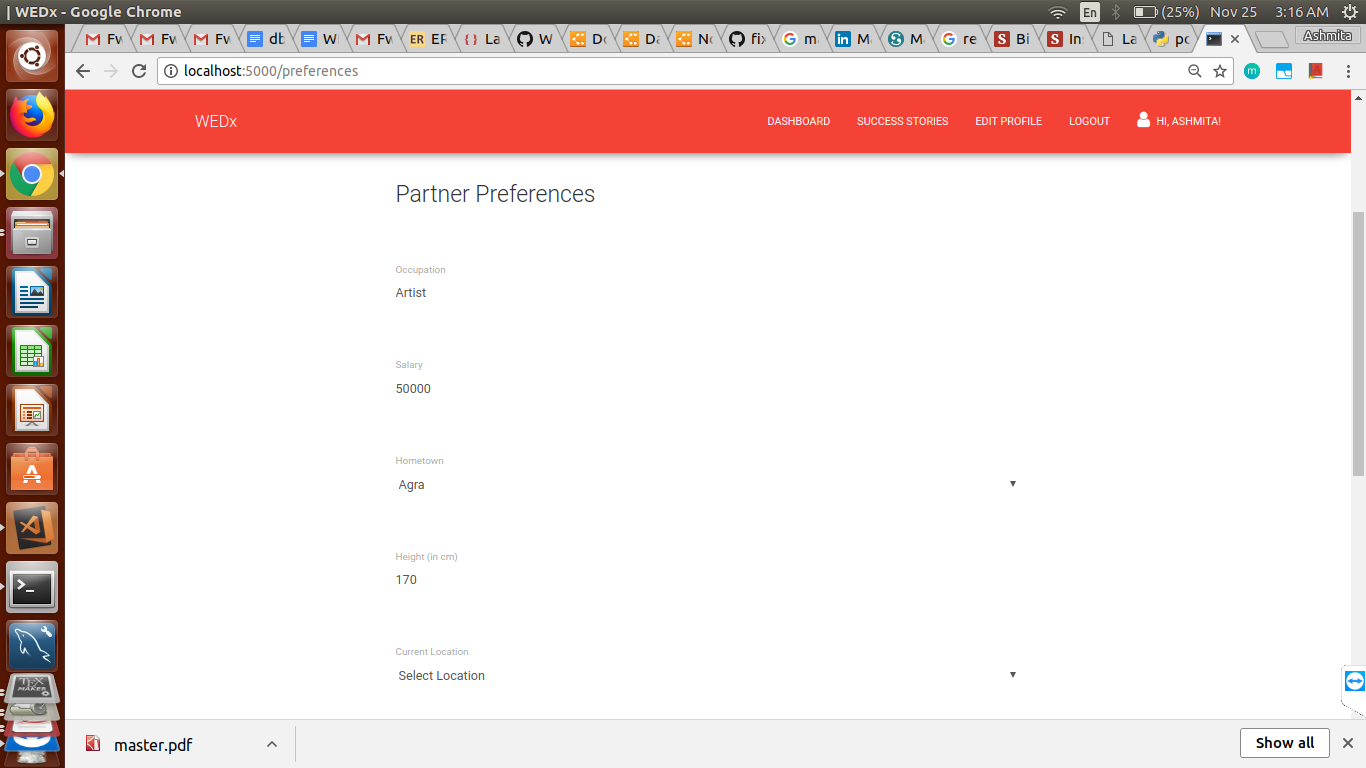
\includegraphics[width=1\textwidth]{sc-8.png}
    \caption{Edit Partner Preferences}
    \label{fig:Edit Partner Preferences}
\end{figure}

\begin{figure}[!htb]
    \centering
    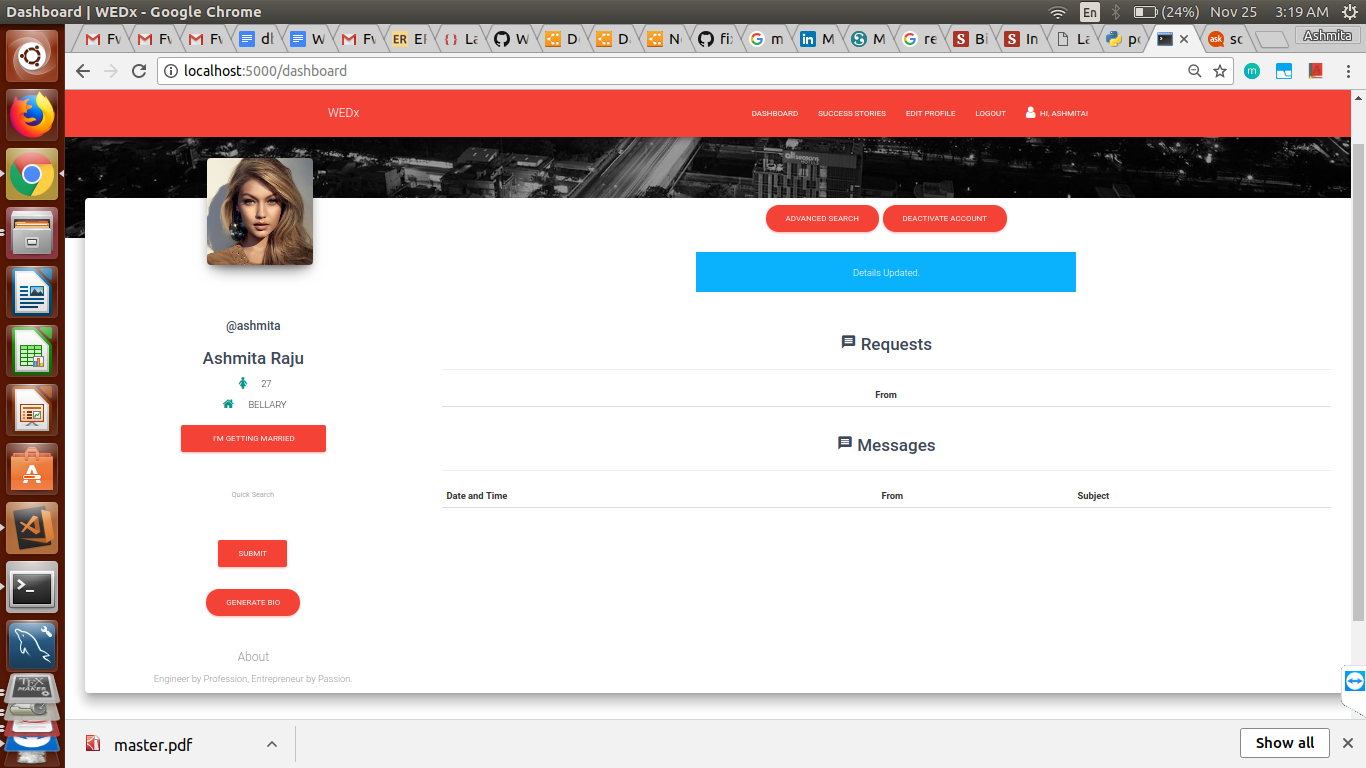
\includegraphics[width=1\textwidth]{sc-9.png}
    \caption{Dashboard}
    \label{fig:Dashboard}
\end{figure}

\begin{figure}[!htb]
    \centering
    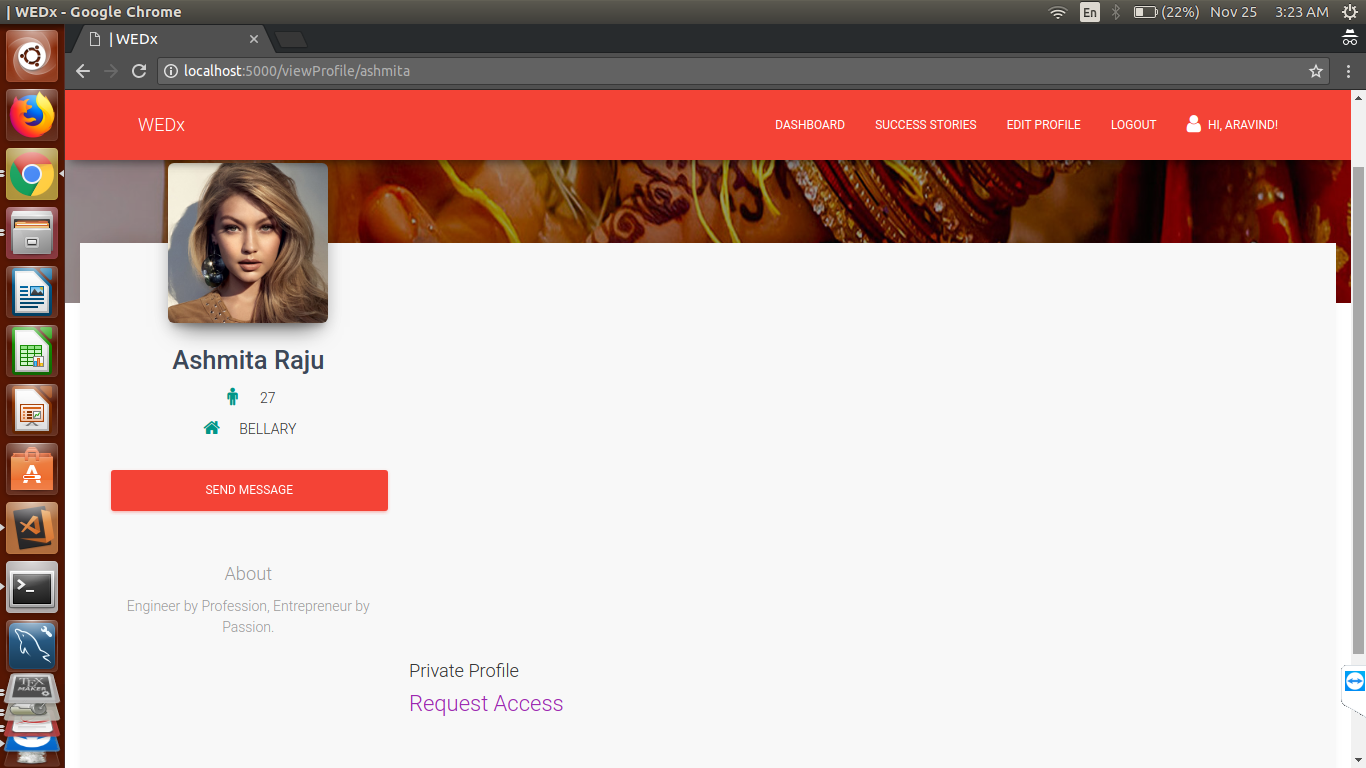
\includegraphics[width=1\textwidth]{sc-10.png}
    \caption{Requesting Access}
    \label{fig:Requesting Access}
\end{figure}

\begin{figure}[!htb]
    \centering
    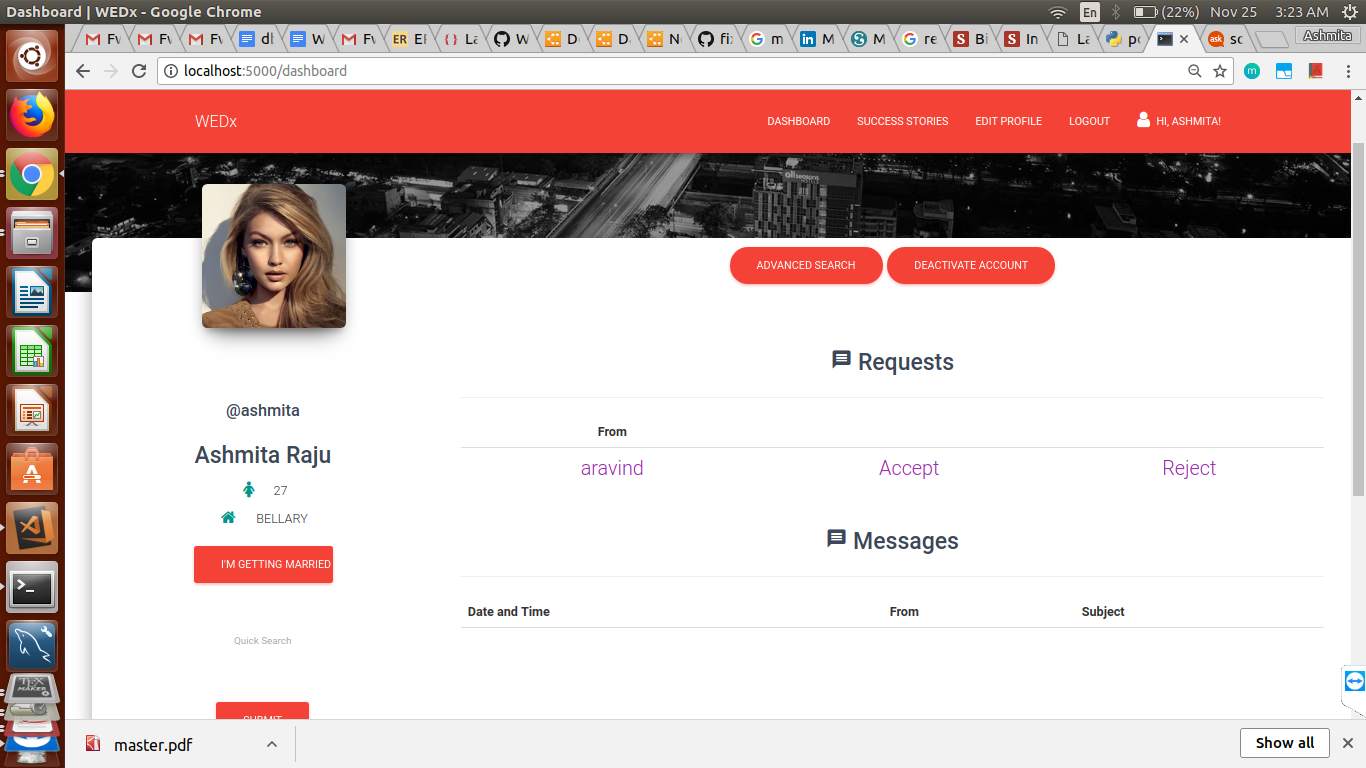
\includegraphics[width=1\textwidth]{sc-11.png}
    \caption{Displaying Requests}
    \label{fig:Displaying Requests}
\end{figure}

\begin{figure}[!htb]
    \centering
    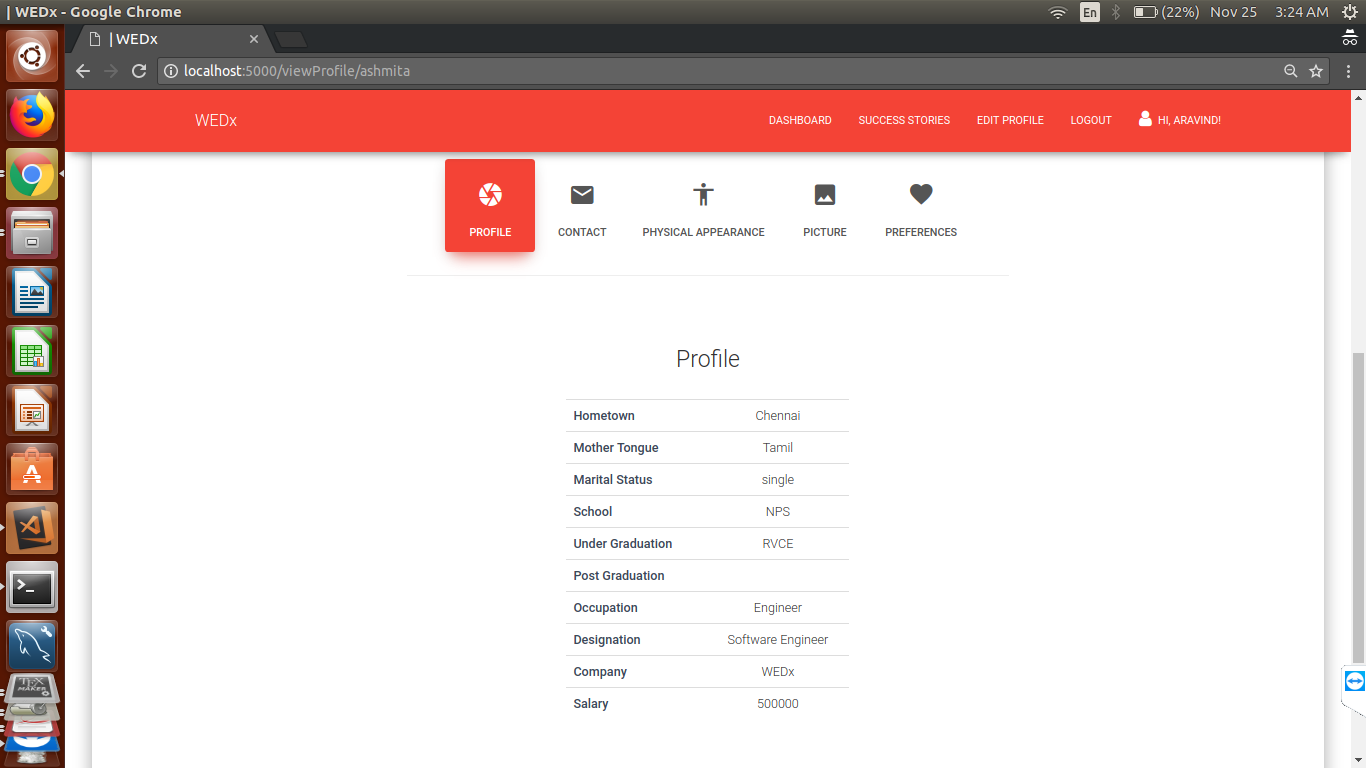
\includegraphics[width=1\textwidth]{sc-12.png}
    \caption{View Profile}
    \label{fig:View Profile}
\end{figure}

\begin{figure}[!htb]
    \centering
    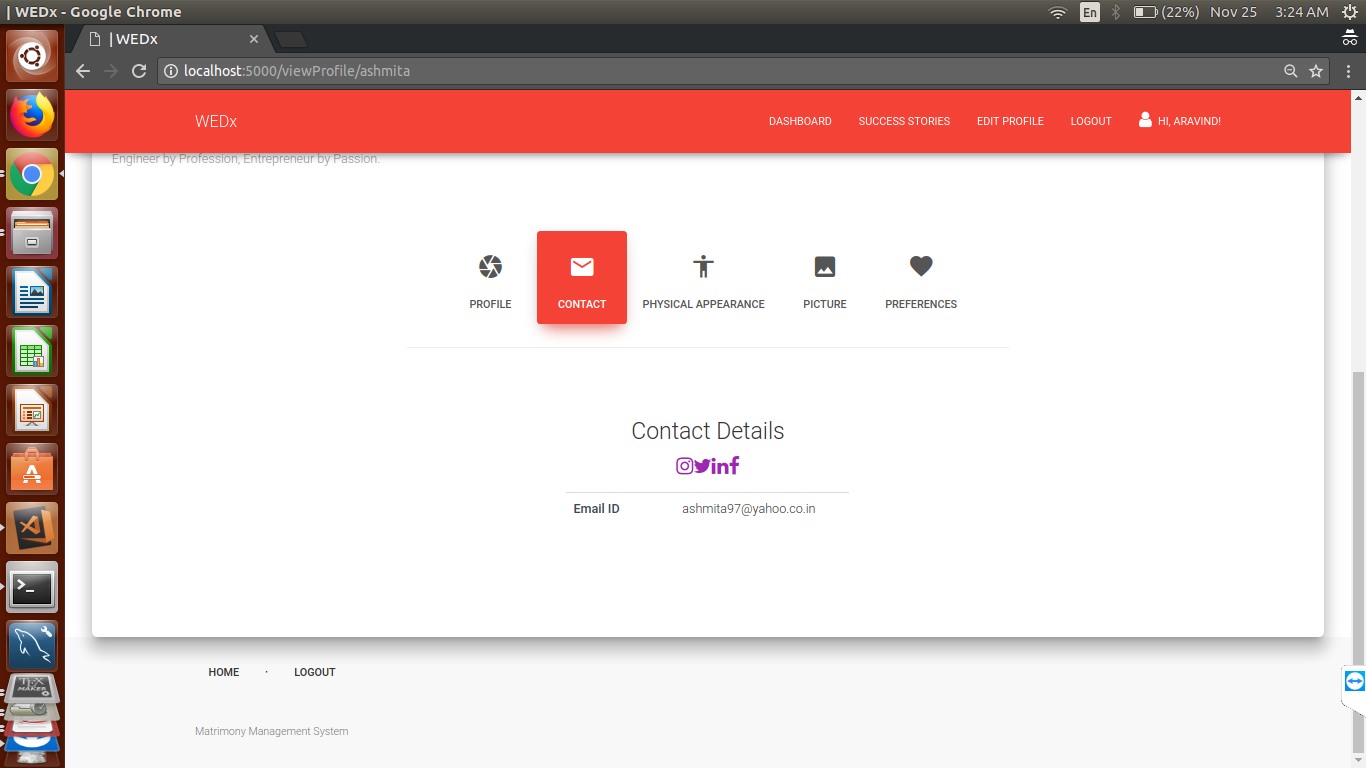
\includegraphics[width=1\textwidth]{sc-13.png}
    \caption{View Profile-2}
    \label{fig:View Profile-2}
\end{figure}

\begin{figure}[!htb]
    \centering
    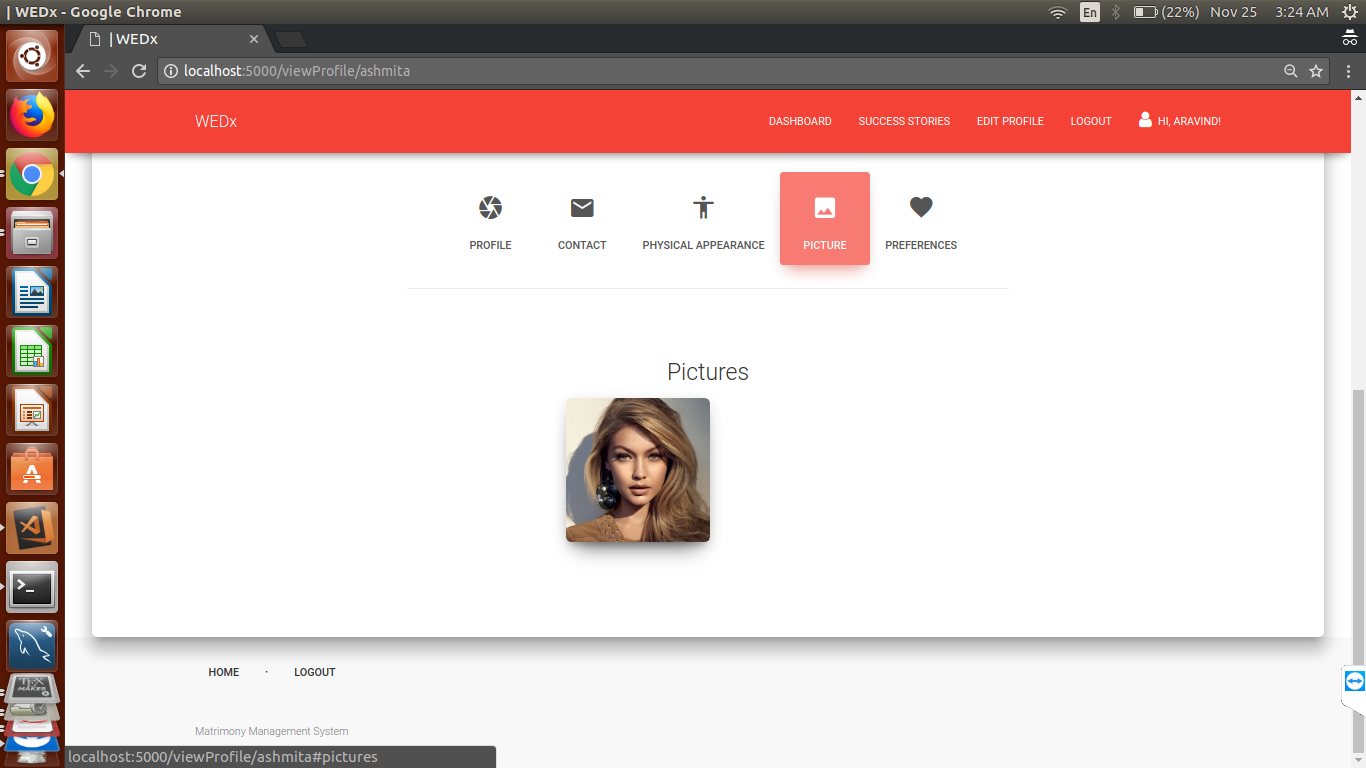
\includegraphics[width=1\textwidth]{sc-14.png}
    \caption{View Profile-3}
    \label{fig:View Profile-3}
\end{figure}

\begin{figure}[!htb]
    \centering
    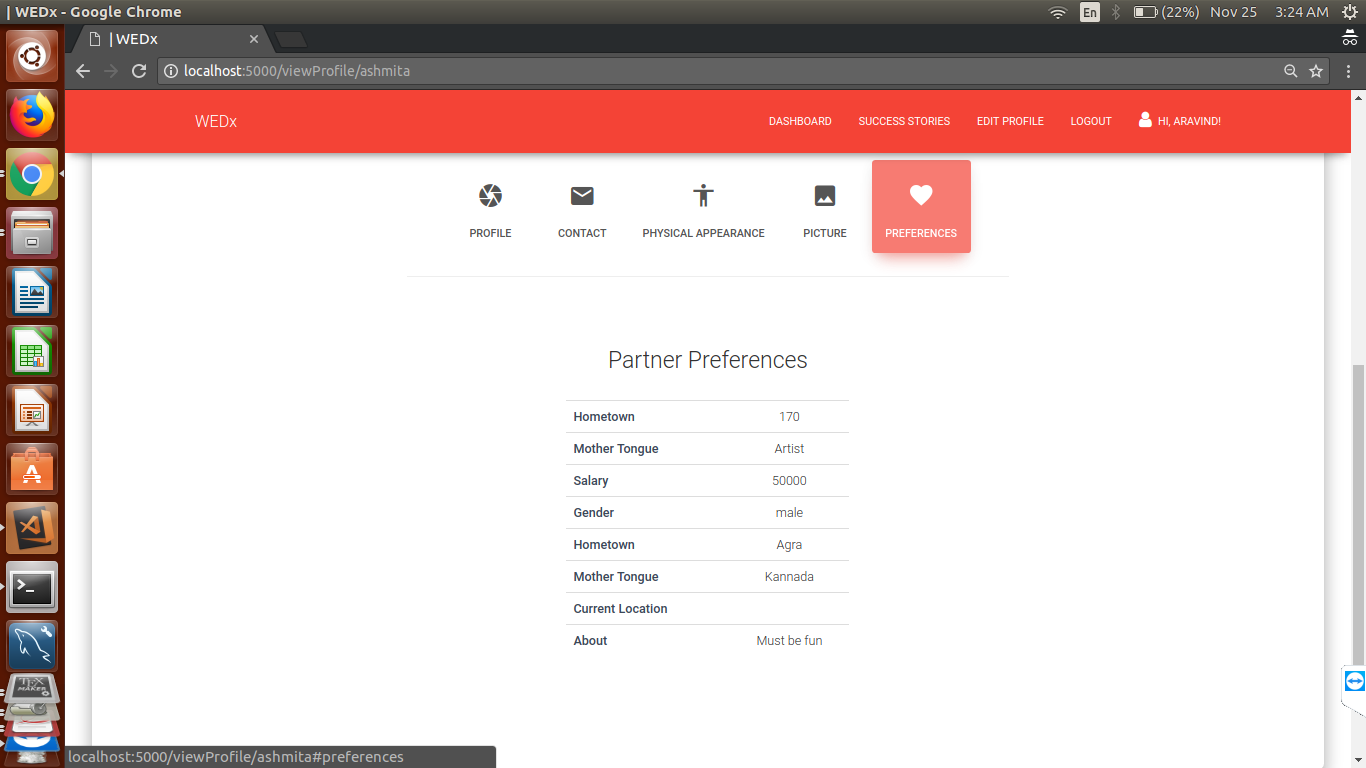
\includegraphics[width=1\textwidth]{sc-15.png}
    \caption{View Profile-4}
    \label{fig:View Profile-4}
\end{figure}

\begin{figure}[!htb]
    \centering
    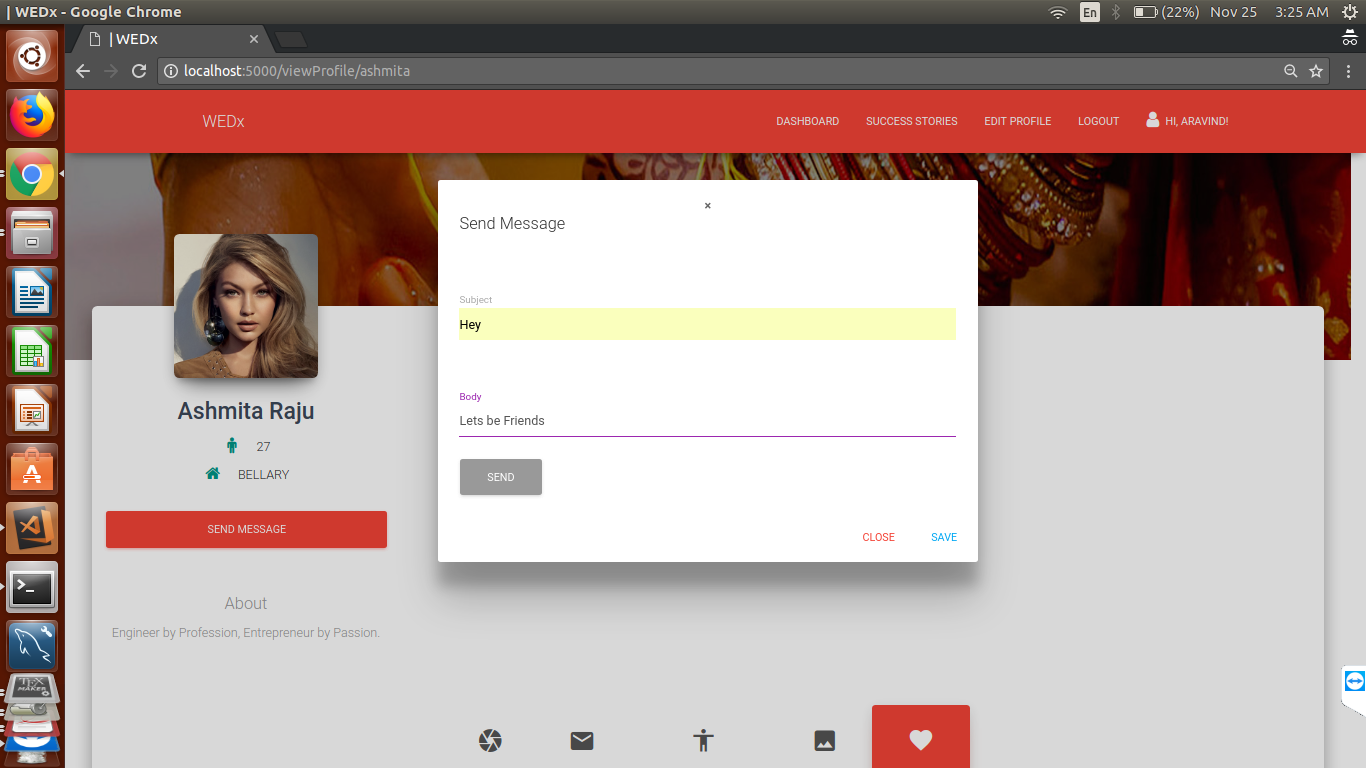
\includegraphics[width=1\textwidth]{sc-16.png}
    \caption{Send Message}
    \label{fig:Send Message}
\end{figure}

\begin{figure}[!htb]
    \centering
    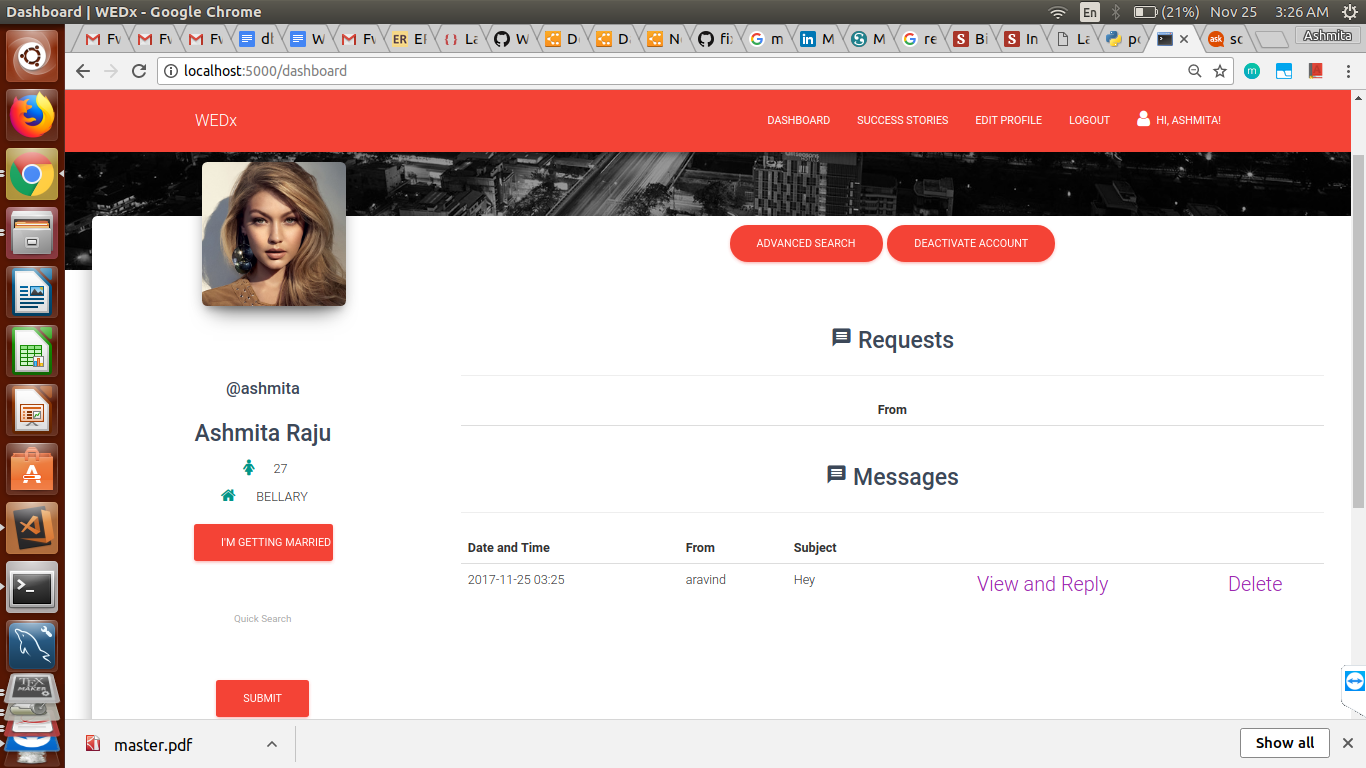
\includegraphics[width=1\textwidth]{sc-17.png}
    \caption{View Message}
    \label{fig:View Message}
\end{figure}

\begin{figure}[!htb]
    \centering
    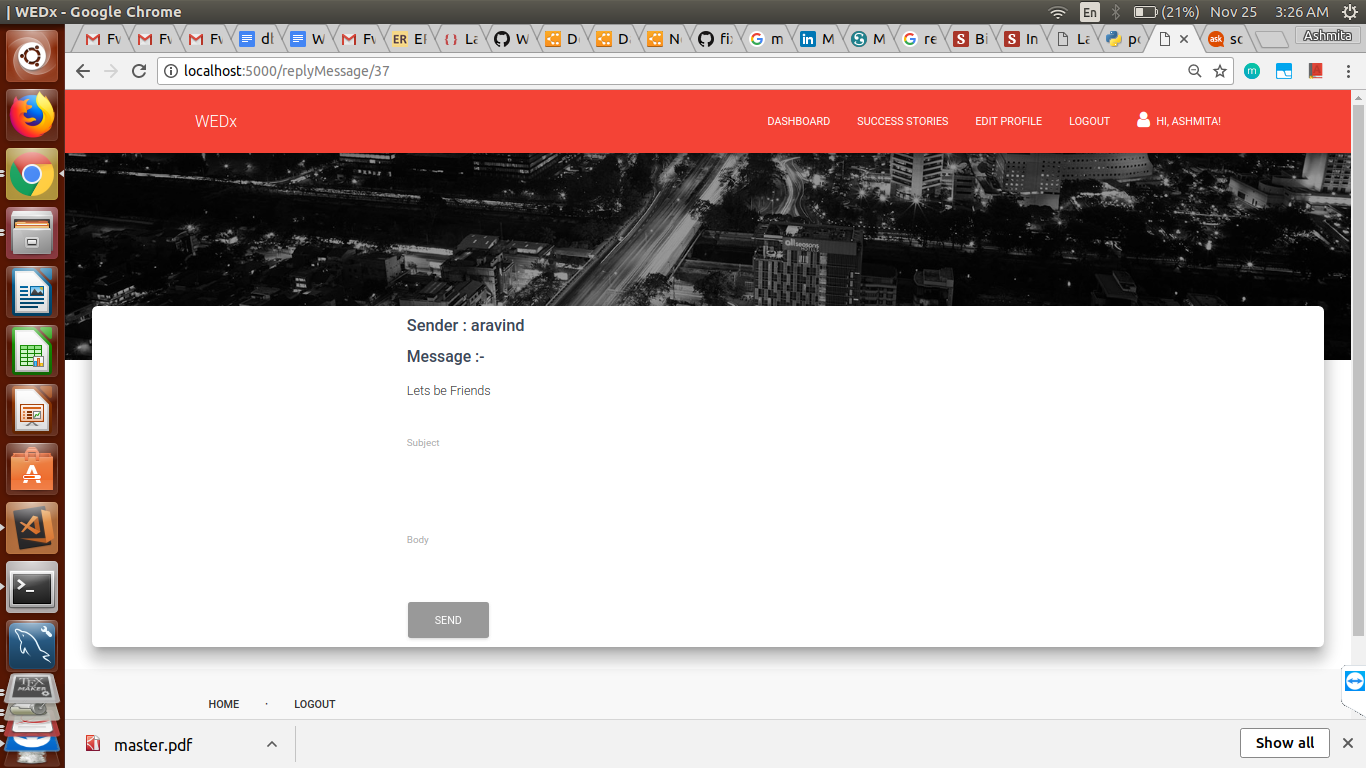
\includegraphics[width=1\textwidth]{sc-18.png}
    \caption{Reply to Message}
    \label{fig:Reply to Message}
\end{figure}

\begin{figure}[!htb]
    \centering
    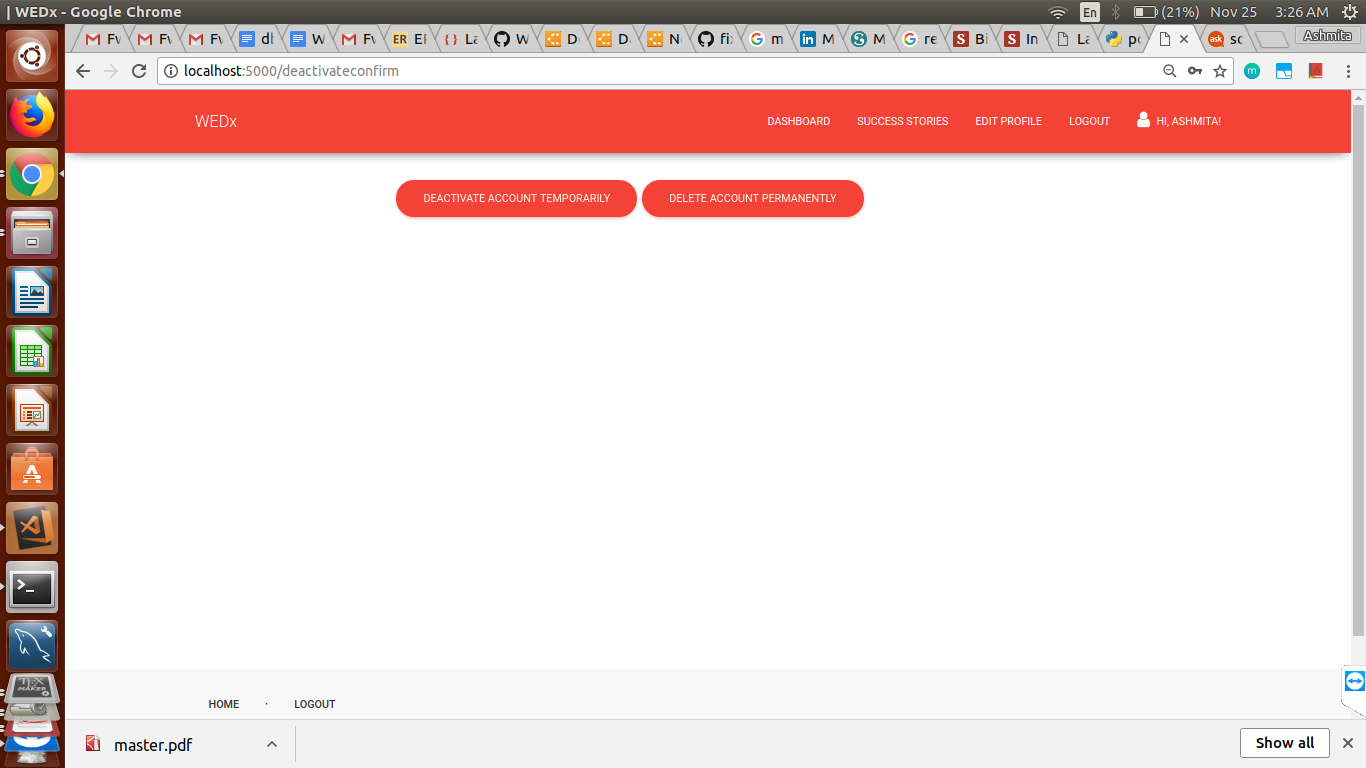
\includegraphics[width=1\textwidth]{sc-19.png}
    \caption{Delete Account}
    \label{fig:Delete Account}
\end{figure}

\begin{figure}[!htb]
    \centering
    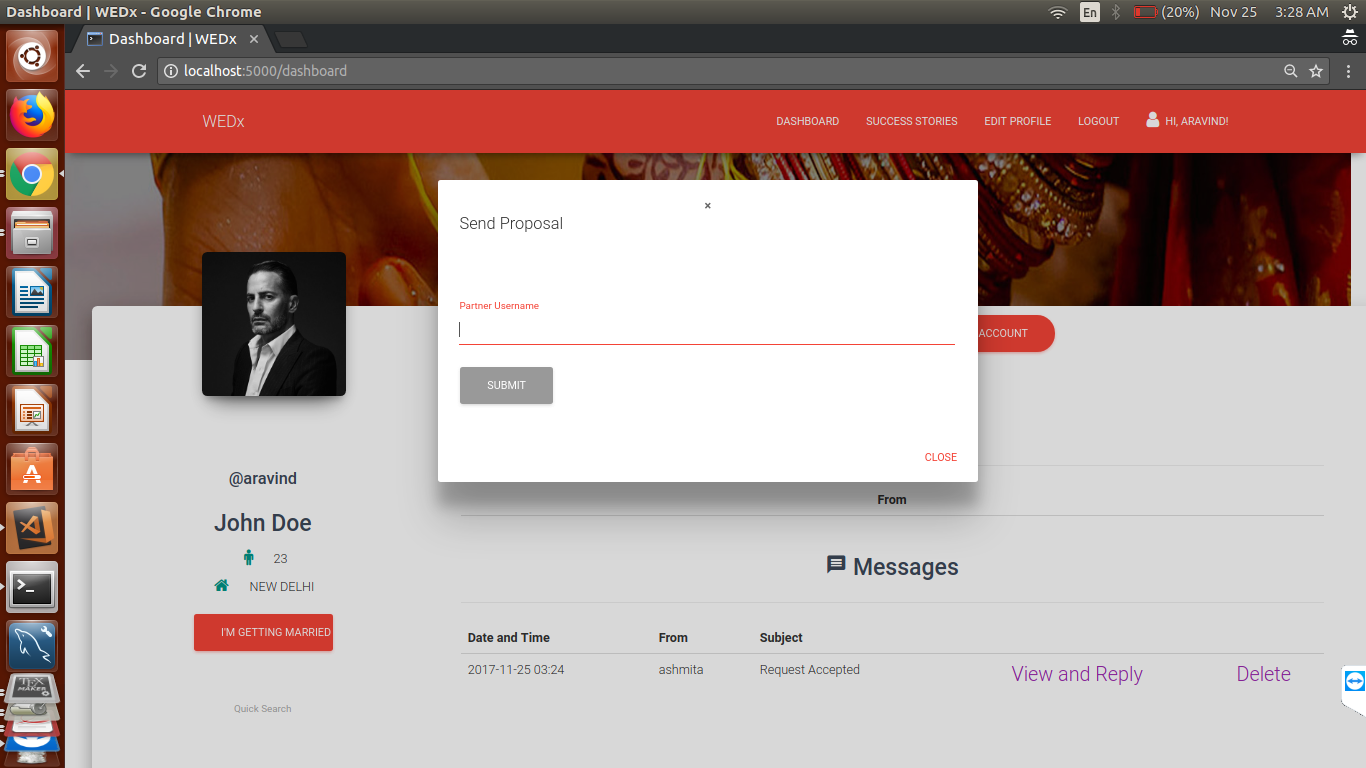
\includegraphics[width=1\textwidth]{sc-20.png}
    \caption{Send Proposal}
    \label{fig:Send Proposal}
\end{figure}


\begin{figure}[!htb]
    \centering
    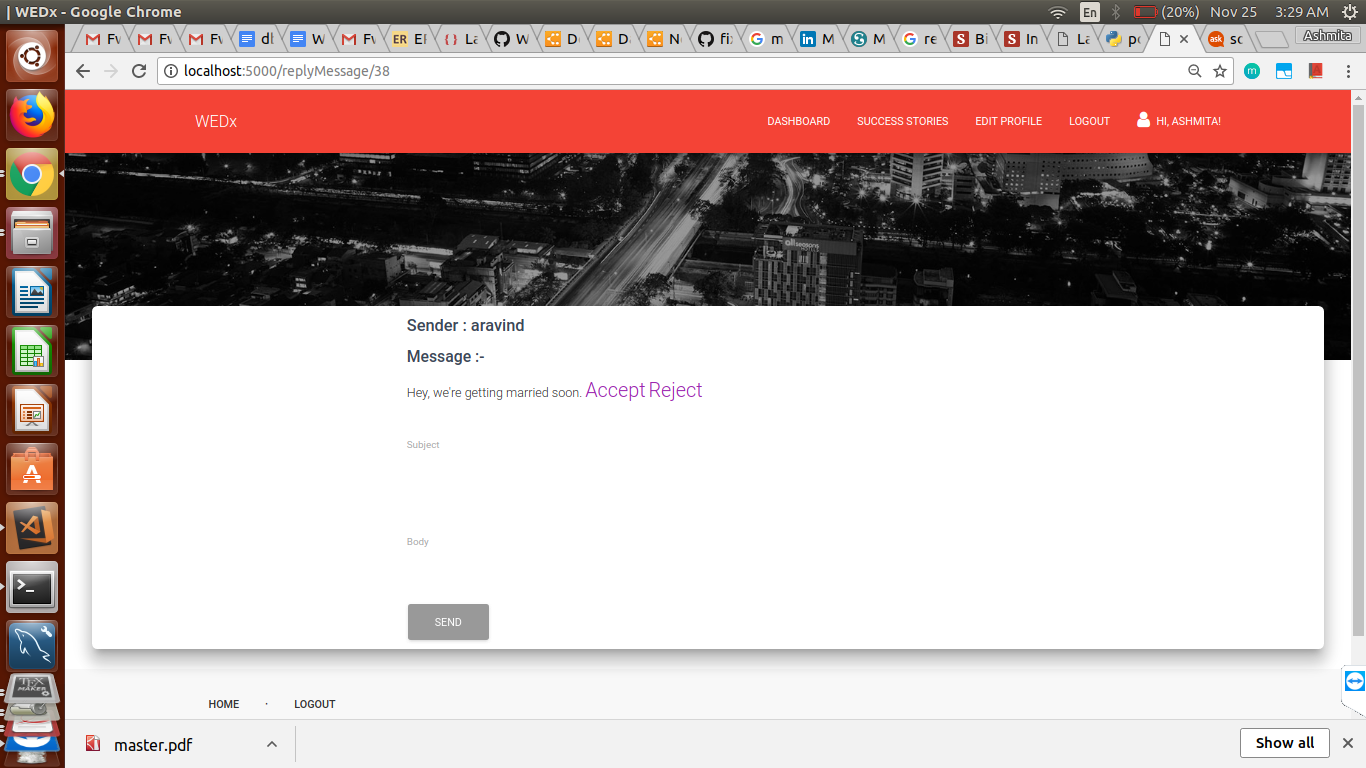
\includegraphics[width=1\textwidth]{sc-22.png}
    \caption{Accept/Reject Proposal}
    \label{fig:Accept/Reject Proposal}
\end{figure}

\begin{figure}[!htb]
    \centering
    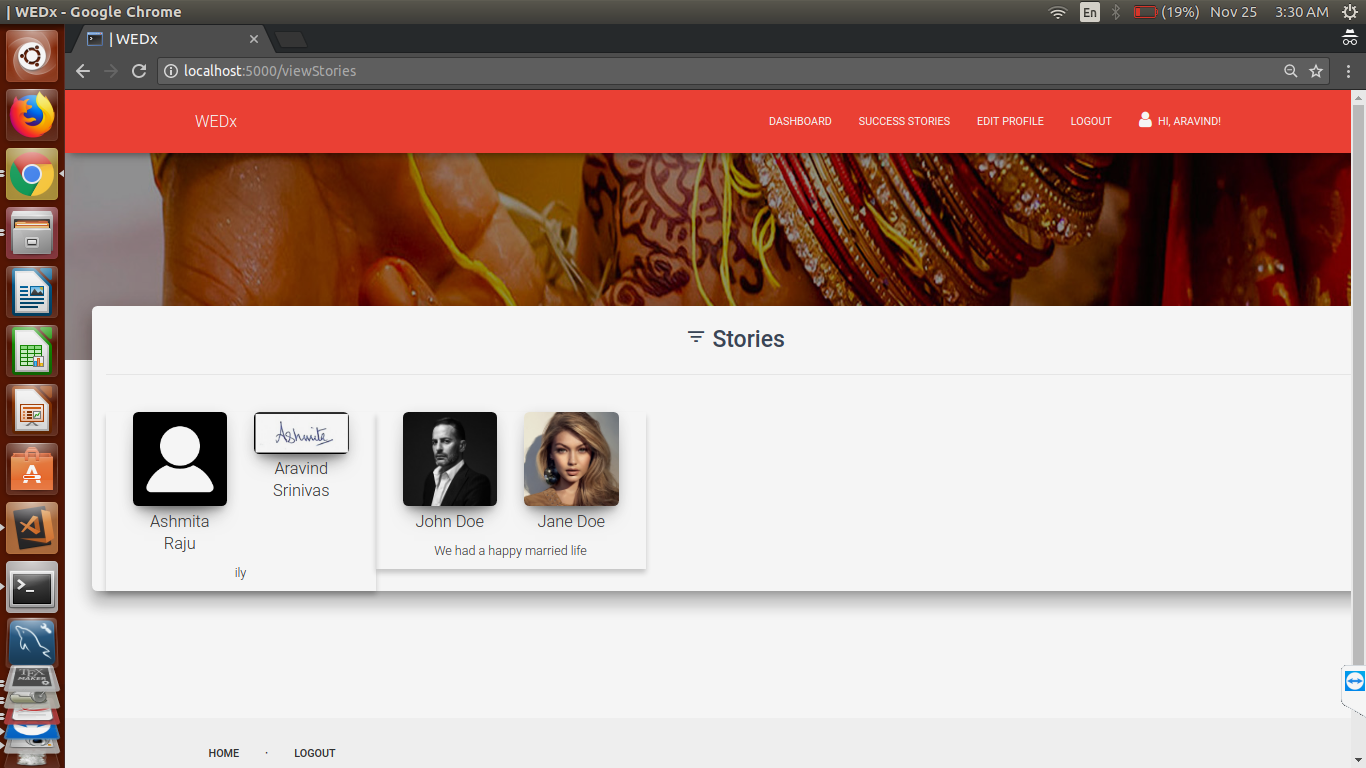
\includegraphics[width=1\textwidth]{sc-23.png}
    \caption{Success Stories}
    \label{fig:Success Stories}
\end{figure}

\begin{figure}[!htb]
    \centering
    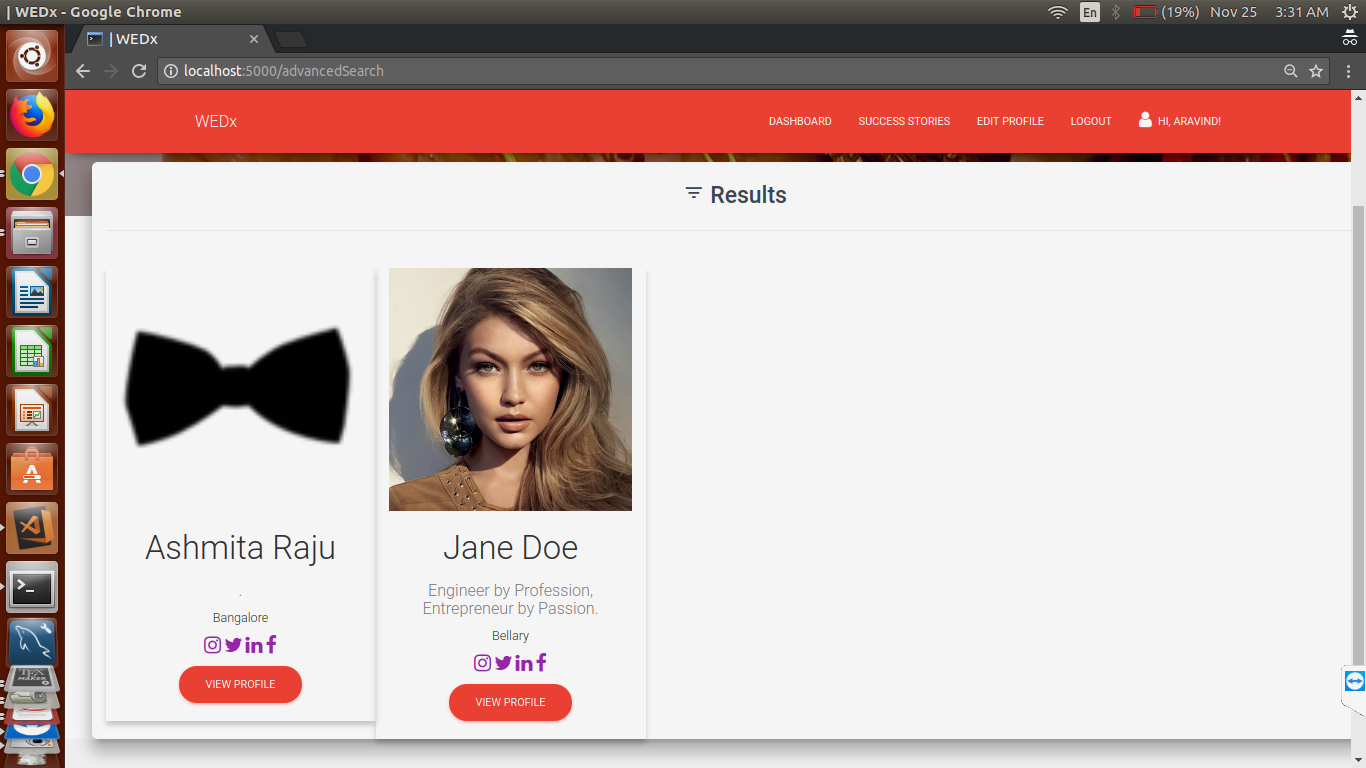
\includegraphics[width=1\textwidth]{sc-24.png}
    \caption{Advanced Search}
    \label{fig:Advanced Search}
\end{figure}



\end{document} 
